% UCL Thesis LaTeX Template
%  (c) Ian Kirker, 2014
% 
% This is a template/skeleton for PhD/MPhil/MRes theses.
%
% It uses a rather split-up file structure because this tends to
%  work well for large, complex documents.
% We suggest using one file per chapter, but you may wish to use more
%  or fewer separate files than that.
% We've also separated out various bits of configuration into their
%  own files, to keep everything neat.
% Note that the \input command just streams in whatever file you give
%  it, while the \include command adds a page break, and does some
%  extra organisation to make compilation faster. Note that you can't
%  use \include inside an \include-d file.
% We suggest using \input for settings and configuration files that
%  you always want to use, and \include for each section of content.
% If you do that, it also means you can use the \includeonly statement
%  to only compile up the section you're currently interested in.
% You might also want to put figures into their own files to be \input.

% For more information on \input and \include, see:
%  http://tex.stackexchange.com/questions/246/when-should-i-use-input-vs-include


% Formatting and binding rules for theses are here: 
%  https://www.ucl.ac.uk/students/exams-and-assessments/research-assessments/format-bind-and-submit-your-thesis-general-guidance

% This package goes first and foremost, because it checks all 
%  your syntax for mistakes and some old-fashioned LaTeX commands.
% Note that normally you should load your documentclass before 
%  packages, because some packages change behaviour based on
%  your document settings.
% Also, for those confused by the RequirePackage here vs usepackage
%  elsewhere, usepackage cannot be used before the documentclass
%  command, while RequirePackage can. That's the only functional
%  difference as far as I'm aware.
\RequirePackage[l2tabu, orthodox]{nag}


% ------ Main document class specification ------
% The draft option here prevents images being inserted,
%  and adds chunky black bars to boxes that are exceeding 
%  the page width (to show that they are).
% The oneside option can optionally be replaced by twoside if
%  you intend to print double-sided. Note that this is
%  *specifically permitted* by the UCL thesis formatting
%  guidelines.
%
% Valid options in terms of type are:
%  phd
%  mres
%  mphil
%\documentclass[12pt,phd,draft,a4paper,oneside]{ucl_thesis}
\documentclass[12pt,mphil,a4paper,oneside]{ucl_thesis}


% Package configuration:
%  LaTeX uses "packages" to add extra commands and features.
%  There are quite a few useful ones, so we've put them in a 
%   separate file.
% -------- Packages --------

% This package just gives you a quick way to dump in some sample text.
% You can remove it -- it's just here for the examples.
\usepackage{blindtext}

% This package means empty pages (pages with no text) won't get stuff
%  like chapter names at the top of the page. It's mostly cosmetic.
\usepackage{emptypage}

% The graphicx package adds the \includegraphics command,
%  which is your basic command for adding a picture.
\usepackage{graphicx}

% The float package improves LaTeX's handling of floats,
%  and also adds the option to *force* LaTeX to put the float
%  HERE, with the [H] option to the float environment.
\usepackage{float}

% The amsmath package enhances the various ways of including
%  maths, including adding the align environment for aligned
%  equations.
\usepackage{amsmath}

% Use these two packages together -- they define symbols
%  for e.g. units that you can use in both text and math mode.
\usepackage{gensymb}
\usepackage{textcomp}
% You may also want the units package for making little
%  fractions for unit specifications.
%\usepackage{units}


% The setspace package lets you use 1.5-sized or double line spacing.
\usepackage{setspace}
\setstretch{1.5}

% That just does body text -- if you want to expand *everything*,
%  including footnotes and tables, use this instead:
%\renewcommand{\baselinestretch}{1.5}


% PGFPlots is either a really clunky or really good way to add graphs
%  into your document, depending on your point of view.
% There's waaaaay too much information on using this to cover here,
%  so, you might want to start here:
%   http://pgfplots.sourceforge.net/
%  or here:
%   http://pgfplots.sourceforge.net/pgfplots.pdf
%\usepackage{pgfplots}
%\pgfplotsset{compat=1.3} % <- this fixed axis labels in the version I was using

% PGFPlotsTable can help you make tables a little more easily than
%  usual in LaTeX.
% If you're going to have to paste data in a lot, I'd suggest using it.
%  You might want to start with the manual, here:
%  http://pgfplots.sourceforge.net/pgfplotstable.pdf
%\usepackage{pgfplotstable}

% These settings are also recommended for using with pgfplotstable.
%\pgfplotstableset{
%	% these columns/<colname>/.style={<options>} things define a style
%	% which applies to <colname> only.
%	empty cells with={--}, % replace empty cells with '--'
%	every head row/.style={before row=\toprule,after row=\midrule},
%	every last row/.style={after row=\bottomrule}
%}


% The mhchem package provides chemistry formula typesetting commands
%  e.g. \ce{H2O}
%\usepackage[version=3]{mhchem}

% And the chemfig package gives a weird command for adding Lewis 
%  diagrams, for e.g. organic molecules
%\usepackage{chemfig}

% The linenumbers command from the lineno package adds line numbers
%  alongside your text that can be useful for discussing edits 
%  in drafts.
% Remove or comment out the command for proper versions.
%\usepackage[modulo]{lineno}
% \linenumbers 


% Alternatively, you can use the ifdraft package to let you add
%  commands that will only be used in draft versions
%\usepackage{ifdraft}

% For example, the following adds a watermark if the draft mode is on.
%\ifdraft{
%  \usepackage{draftwatermark}
%  \SetWatermarkText{\shortstack{\textsc{Draft Mode}\\ \strut \\ \strut \\ \strut}}
%  \SetWatermarkScale{0.5}
%  \SetWatermarkAngle{90}
%}


% The multirow package adds the option to make cells span 
%  rows in tables.
\usepackage{multirow}


% Subfig allows you to create figures within figures, to, for example,
%  make a single figure with 4 individually labeled and referenceable
%  sub-figures.
% It's quite fiddly to use, so check the documentation.
%\usepackage{subfig}

% The natbib package allows book-type citations commonly used in
%  longer works, and less commonly in science articles (IME).
% e.g. (Saucer et al., 1993) rather than [1]
% More details are here: http://merkel.zoneo.net/Latex/natbib.php
%\usepackage{natbib}

% The bibentry package (along with the \nobibliography* command)
%  allows putting full reference lines inline.
%  See: 
%   http://tex.stackexchange.com/questions/2905/how-can-i-list-references-from-bibtex-file-in-line-with-commentary
\usepackage{bibentry} 

% The isorot package allows you to put things sideways 
%  (or indeed, at any angle) on a page.
% This can be useful for wide graphs or other figures.
%\usepackage{isorot}

% The caption package adds more options for caption formatting.
% This set-up makes hanging labels, makes the caption text smaller
%  than the body text, and makes the label bold.
% Highly recommended.
\usepackage[format=hang,font=small,labelfont=bf]{caption}

% If you're getting into defining your own commands, you might want
%  to check out the etoolbox package -- it defines a few commands
%  that can make it easier to make commands robust.
\usepackage{etoolbox}

\usepackage{caption}
\usepackage{subcaption}

% Sets up links within your document, for e.g. contents page entries
%  and references, and also PDF metadata.
% You should edit this!
\input{LinksAndMetadata}

% And then some settings in separate files.
\input{FloatSettings} % For things like figures and tables
\bibliographystyle{ieeetr}   % For bibliographies

% These control how many number sections your subsections will take
%    e.g. Section 2.3.1.5.6.3
%  and how many of those will get put into the contents pages.
\setcounter{secnumdepth}{3}
\setcounter{tocdepth}{3}


\begin{document}

\nobibliography*
% ^-- This is a dumb trick that works with the bibentry package to let
%  you put bibliography entries whereever you like.
% I used this to put references to papers a chapter's work was 
%  published in at the end of that chapter.
% For more information, see: http://stefaanlippens.net/bibentry

% If you haven't finished making your full BibTex file yet, you
%  might find this useful -- it'll just replace all your
%  citations with little superscript notes.
% Uncomment to use.
%\renewcommand{\cite}[1]{\emph{\textsuperscript{[#1]}}}

% At last, content! Remember filenames are case-sensitive and 
%  *must not* include spaces.
% I may change the way this is done in a future version, 
%  but given that some people needed it, if you need a different degree title 
%  (e.g. Master of Science, Master in Science, Master of Arts, etc)
%  uncomment the following 3 lines and set as appropriate (this *has* to be before \maketitle)
% \makeatletter
% \renewcommand {\@degree@string} {Master of Things}
% \makeatother

\title{Structural Uncertainty in Cardiovascular CFD models}
\author{Thanh Trung Mai}
\department{Medical Physics and Biomedical Engineering}

\maketitle
\makedeclaration

\begin{abstract} % 300 word limit
My research is about stuff.

It begins with a study of some stuff, and then some other stuff and things.

There is a 300-word limit on your abstract.
\end{abstract}

\begin{impactstatement}

UCL theses now have to include an impact statement. \textit{(I think for REF reasons?)} The following text is the description from the guide linked from the formatting and submission website of what that involves. (Link to the guide: {\scriptsize \url{http://www.grad.ucl.ac.uk/essinfo/docs/Impact-Statement-Guidance-Notes-for-Research-Students-and-Supervisors.pdf}})

\begin{quote}
The statement should describe, in no more than 500 words, how the expertise, knowledge, analysis,
discovery or insight presented in your thesis could be put to a beneficial use. Consider benefits both
inside and outside academia and the ways in which these benefits could be brought about.

The benefits inside academia could be to the discipline and future scholarship, research methods or
methodology, the curriculum; they might be within your research area and potentially within other
research areas.

The benefits outside academia could occur to commercial activity, social enterprise, professional
practice, clinical use, public health, public policy design, public service delivery, laws, public
discourse, culture, the quality of the environment or quality of life.

The impact could occur locally, regionally, nationally or internationally, to individuals, communities or
organisations and could be immediate or occur incrementally, in the context of a broader field of
research, over many years, decades or longer.

Impact could be brought about through disseminating outputs (either in scholarly journals or
elsewhere such as specialist or mainstream media), education, public engagement, translational
research, commercial and social enterprise activity, engaging with public policy makers and public
service delivery practitioners, influencing ministers, collaborating with academics and non-academics
etc.

Further information including a searchable list of hundreds of examples of UCL impact outside of
academia please see \url{https://www.ucl.ac.uk/impact/}. For thousands more examples, please see
\url{http://results.ref.ac.uk/Results/SelectUoa}.
\end{quote}
\end{impactstatement}

\begin{acknowledgements}
Acknowledge all the things!
\end{acknowledgements}

\setcounter{tocdepth}{2} 
% Setting this higher means you get contents entries for
%  more minor section headers.

\tableofcontents
\listoffigures
\listoftables


\chapter{Introduction}
\label{chapterlabel1}

Computational models are usually constructed by applying an established physical principle that relate time-dependent variables which describe the state of the system to measured model parameters. This makes the models suitable to study complex dynamic processes and systems and predict the future behaviour of the system.\par

Over the past decade, the use of computational modelling in the cardiovascular research has showed numerous different approaches that could be benefitial for clinical use. The use of computational models with patient-specific inputs calculates in both, space and time, variables such as flow, velocity gradients, pressures, wall shear stress and vessel motion displacement which can be helpful in decision-making processes. Additionally, the models can be parametrically modified to assist clinicians in investigating the outcome of various treatment methods, following a systematic approach.

Despite the numerous effort in making cardiovascular models viable for the clinical support, there are still numerous major challenges for these models to be used in the clinic. Often, patient-specific data in certain areas is difficult or impossible to obtain, thus simplifications of real-life processes would be necessary. Furthermore, due to this lack of data, often models are run in an "idealised" scenario which can introduce structural uncertainty into the results, which is the error stemming from inadequate assumptions. Lastly, there is a very little consensus in the cardiovascular modelling on the assessment of these uncertainties and variability. Nevertheless, these are critical to gain trust and acceptance in the clinic  \par

In this report, the background to cardiovascular modelling will be introduced and the process of verification, validation and uncertainty quantification of cardiovascular models will be explained. In the literature review, the different methods to assess uncertainties will be explained and current work in the cardiovascular modelling field  will be reviewed. Then a conceptual modelling framework to identify the structural uncertainty areas will be introduced.
\chapter{Background}
\label{chapterlabel2}
In this chapter, background related to the physiology of the cardiovascular system and computational fluid dynamics in this field will be introduced. Additionally, the process of verification, validation and uncertainty quantification will be explained.


\section{Cardiovascular system}
The cardiovascular system, also called the circulatory system, is a closed-loop system composed by the heart, blood vessels and blood. It uses blood as the medium to distribute oxygen and nutrients to all body tissues and dispose of carbon-dioxide and metabolic waste to lungs and excretory organs. Additionally, the secondary function of the system is to redistribute bioactive agents and hormones throughout the body, and regulate the body temperature \cite{Levick2010Introduction5ed}.\par

The heart is a muscular organ that  pumps the blood into the blood vessels to distribute it around the body. It is located in between the lungs above the sternum. The heart is divided into two sides and each side is divided further into two chambers (as seen on Figure \ref{fig:heart}. The top chambers are the atria and the bottom ones are the ventricles. The wall of the heart are composed of cardiac muscle which produce contraction that pump the blood into the arteries \cite{aaronson2012cardiovascular,tortora2017introduction}. \par

The system is divided into two circulatory loops with the heart at the center, a pulmonary circulation and systemic circulation. In the pulmonary circulation, the deoxygenated blood is pumped from the heart's right ventricle into the pulmonary artery, where the blood is transported into the lungs where an oxygen exchange occurs. The blood then returns to the left atrium, passes through the left ventricle into the systematic circulation\cite{Levick2010Introduction5ed,tortora2017introduction}. \par


\begin{figure}[ht!]
  \centering
  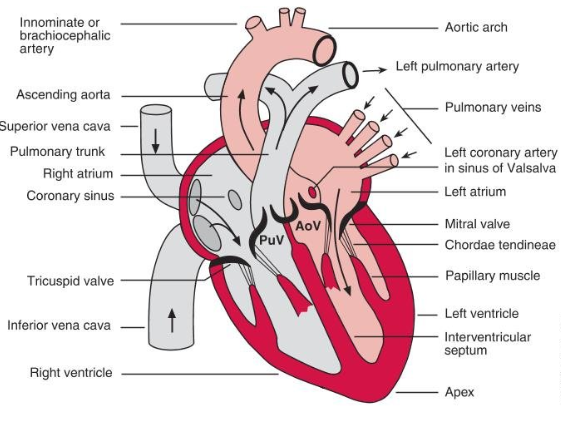
\includegraphics[width=0.6\textwidth]{Figures/heart.PNG}
  \caption{Structure of the heart and connection to the major veins and arteries \cite{Levick2010Introduction5ed}.}
  \label{fig:heart}
\end{figure}


Blood vessels in the system are responsible to deliver the blood into organs and tissue. The blood is driven into the aorta from there it flows into the major arteries, which then deliver blood to the major regions and organs. The arteries can further branch out and then they converge into veins which transport the blood back into the heart \cite{Levick2010Introduction5ed}.\par

\section{Computational Modelling for cardiovascular applications}
Computational models have been often used to study the haemodynamics of the a system. These have been often used for hypothesis creation, mechanistic understanding, device evaluation or educational purposes. With better imaging modalities and improved devices to obtain patient measurements, patient-specific modelling has emerged, showcasing their predictive power and their capability of being used in diagnosis or predictive medicine was considered. Where the models are made tailored to the patient anatomy.\par
\begin{figure}
    \centering
    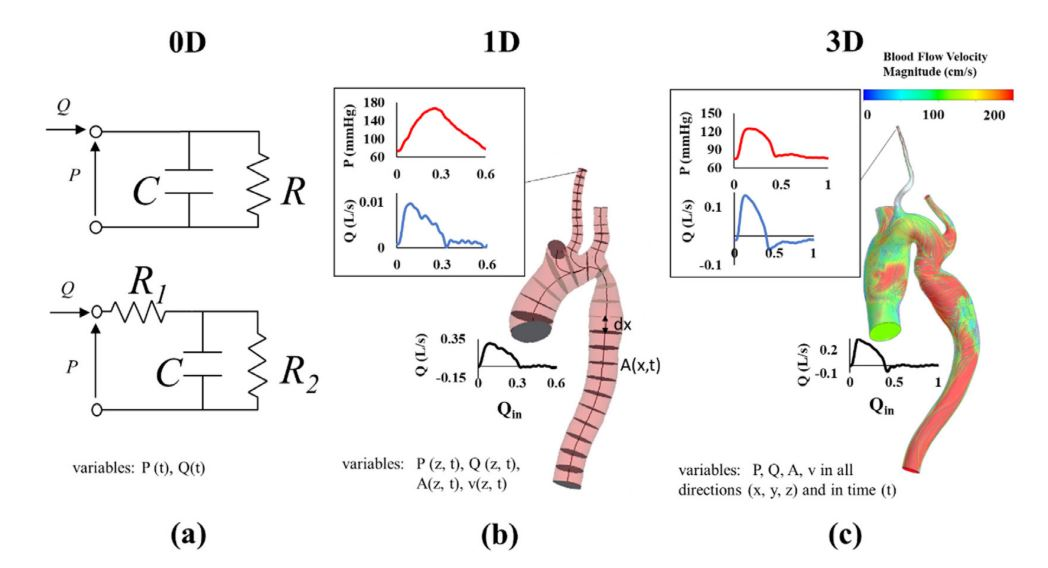
\includegraphics[width=\textwidth]{Figures/CardioMod.JPG}
    \caption{Illustration of \textbf{a)} zero-dimensional, \textbf{b)} one-dimensional and \textbf{c)} three dimensional vascular models \cite{Hose2019CardiovascularNext}}
    \label{fig:CardioMod}
\end{figure}

Cardiovascular models can be categorised by their dimension as seen on Figure \ref{fig:CardioMod}. Zero-dimensional (0D), or lumped parameter models, divide the system into individual components and represent effects through lumped parameters. The governing equations are ordinary differential equations. Lumped parameter models of the circulation are analogous to an electrical circuit where the physiological variables pressure, volume and flow are equivalent to to voltage, charge and current. 0D models can be used to simulate the global haemodynamic in the whole circulation system \cite{Zhou2019APressure} and can be extended to include biochemical and biomechanical processes \cite{Hose2019CardiovascularNext}. \par

One dimensional models (1D) are distributed parameter models, which can represent distributed properties along the vessel axis. These models are represented using partial differential equations in time and one spatial dimension and they are used to study pulse wave transmission \cite{Zhou2019APressure, Hose2019CardiovascularNext}. \par 

\subsection{Computational Fluid Dynamics}
A three-dimensional analysis of the flow in a patient-specific anatomy yields spatial and temporal on variables such as flow, pressure, wall shear stress or wall displacemet. The governing equations of the flow are the Navier-Stokes equations (\ref{eq:n_s}), which describe the conservation of momentum of a fluid.
% rewrite
Thus, the flow can be calculated in conjunction with the conservation of mass equation (\ref{eq:con} ):
\begin{equation}
\frac{\partial \rho}{\partial t}+\nabla \cdot (\rho U) = 0 \\
\label{eq:con}
\end{equation}
\begin{equation}
\frac{\partial (\rho U)}{\partial t}+\nabla \cdot (\rho U \times U) = -\nabla p + \nabla \cdot \tau + S_{M}
\label{eq:n_s}
\end{equation}
where, $p$ and $\tau$ are the pressure and stress tensor, respectively and $U$ is the velocity of the flow. The term $S_M$ refers to external forces to the system. \par

\subsection{Patient-specific data}
In order to create image-based patient-specific haemodynamics models, it is necessary to obtain geometry and flow data. \par

Imaging techniques such a computed tomography (CT) can be used to obtain a number of image slices which would then be used to reconstruct the 3D model of the tissue and organs of the patient. The method  uses ionising radiation which benefits from high spatial resolution and high penetration depth. However, CT scanning often has limited sensitivity and also exposes the patient to radiation \cite{Saremi2015CoronaryCT}. An alternative method to obtain the geometry can be magnetic resonance imaging (MRI) which uses the principles of electromagnetism to capture the images. It yields the images based on the radiofrequency of the tissue, generated by the hydrogen atoms within the tissues. Using MRI, the patient is not exposed to radiation or contrast agents. However, in comparison with the CT images, MRI has lower spatial resolution and is much more time-consuming to acquire whole 3D stack of images \cite{Maurovich-Horvat2012DifferentiationHearts, Karmonik2008ComputationalRates}.\par

Other patient-specific data such as volumetric flow, pressure  or wall displacement data has to be obtained in order to create accurate haemodynamic models. There are numerous ways how these can be obtained, both invasively and non-invasively. While invasive methods can provide accurate measurements through the application of different sensors, their application is restricted and use carefully considered. Several non-invasive imaging techniques can be employed. Doppler echocardiography or phase contrast (PC) MRI have shown to be a good method for obtaining flow measurements non-invasively \cite{Whitlock2015NoninvasiveAorta}. For wall, the time-resolved images must be obtained; this can be done using electrocardiogram (ECG) coupled with CT or 4D MRI data for example \cite{Bonfanti2017ComputationalData,Alimohammadi2015AorticUnderstanding}.

\subsection{Modelling assumptions}
Different modelling assumptions are used to explore computationally cardiovascular conditions. These will be briefly presented bellow.

\subsubsection{Boundary conditions}
Boundary conditions are essential in order to obtain realistic results.  \par

A number of inlet conditions can be imposed. The velocity profile can be considered either as uniform or as parabolic profile (Poiseuille or Womersley) \cite{Steinman2019HowVariability, Alimohammadi2015AorticUnderstanding}. If patient-specific data on the flow rates are absent, usually a necessary simplification is necessary where the flow rate is taken from previous studies or averaged from a published cohort. Another method would be scaling the waveform shape from literature by the vessel diameter \cite{Morris2016ComputationalMedicine}. \par

At the outlets, the simplest boundary condition to apply is constant pressure outlet (usually zero). This is usually done in rigid-wall simulation, where the pressure drop drives the flow rather then the absolute pressure. Another approach applies a scaling law to the outlet, where the pressure at the outlet could depend on the outlet's diameter or branch length which shows to have much superior estimation to the zero-pressure assumption \cite{Pirola2017OnDynamics, Les2010QuantificationDynamics}. \par

Most simulations assume the walls of the arteries to be rigid with a no-slip condition. However, as the arterial wall is compliant,  a number of studies suggest that the wall motion is an important factor that could influence the variables of interest \cite{Alimohammadi2017, Bonfanti2018AInteraction}. One of the method common method of modelling the wall displacement is using the fluid-structure interaction where the wall is modelled as an elastic wall where it expands with pressure changes. However, in comparison to the rigid wall simulation, this method is computationally expensive \cite{Steinman2012AssumptionsHemodynamics}.

\subsubsection{Blood viscosity model}
Blood is a complex fluid composed of red and white blood cells and platelets in plasma. While blood exhibits non-Newtonian properties, many of the haemodynamic models assume blood as a Newtonian fluid in large arteries. While the strain rates in these vessels are very low \cite{Fung1997BiomechanicsCirculation}, the Newtonian fluid does not take into account the shear-thinning properties of blood. By increasing the shear rate on the blood, the viscosity decreases (as seen in Figure \ref{fig:visc}) as a result of the disaggregation and the deformation of red blood cells \cite{Gijsen1999TheModel,Cho1991EffectsFlows}. Simple non-Newtonian models, such as Carreau-Yasuda or Casson, have been used to approximate the complex behaviour of the blood and to improve the study of the properties of the blood in vessels  \cite{Alimohammadi2015PredictingApproach}. \par

\begin{figure}[ht!]
\centering
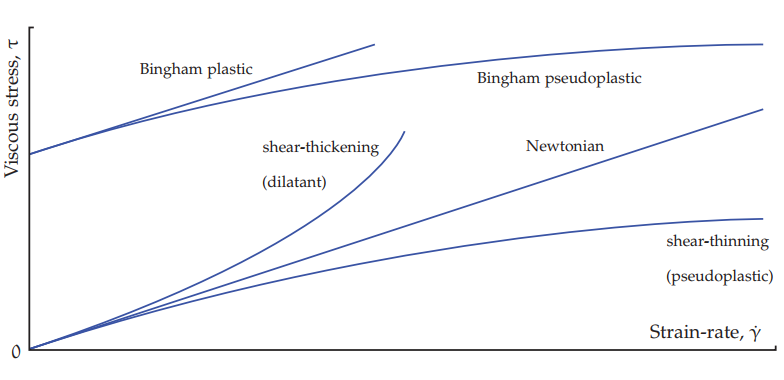
\includegraphics[width=\textwidth]{Figures/viscosity}
\caption{The relation of viscous stress and strain-rate, a comparison of Newtonian and non-Newtonian models \cite{Gabriel2017THEGROWTH}}
\label{fig:visc}
\end{figure}

\subsubsection{Flow models}
Another important consideration whether the flow is laminar, transitional or turbulent \cite{Morris2016ComputationalMedicine}. Turbulent flow introduces random fluctuations in the velocity resulting in turbulent eddies and dissipation of energy in the flow \cite{DongenF.N.vandeVosse2003CardiovascularMechanics}. The Reynold's number $Re$ which is the ratio of the inertial and viscous forces is used to determine the flow regime: 
\begin{equation}
Re = \frac{\rho UD}{\mu}
\end{equation}
Where D is the characteristic length, U is the velocity, $\rho$ is the density and $\mu$ is the viscosity.\par

The transition to turbulence occurs at a critical Reynold's number ($Re_c$) of around 2000. However, as turbulence takes time to develop, pulsatile flow that occurs in arteries, has higher $Re_c$ which increases with the Womersley number (the ratio of transient inertial forces to viscous forces) \cite{Alimohammadi2015PredictingApproach}. A number of studies on the flow conditions in the arteries have found that $Re_c$ varies in the range 2700-15000 and that the maximum Reynolds number in arteries is up to 3700. Therefore, a majority of studies implement the flow as a laminar model \cite{Ku1997BLOODARTERIES}. \par


\section{Verification, validation and uncertainty quantification (VVUQ)}
While computational models can provide a framework to study the complex processes, it is necessary to question the credibility of computational models. The process of assessing models is done in three stages, verification, validation and uncertainty quantification (VVUQ), where different aspects of the models are evaluated. \par

Verification is the assessment of the mathematical and computational reliability. This can involve the assessment of the software quality, design and code review or the numerical analysis of the algorithm used in the code and it's properties (i.e. symmetry, stability, conservation, convergence, etc.). The error of the model is evaluated by validation which compares the numerical results of the model with the true value obtained from the experiments. Lastly the uncertainty quantification determines how variations in the numerical and physical parameters affect simulation outcomes \cite{VerificationASME}.

In other engineering fields, proper guidelines of VVUQ are established for the assessment of the computational models credibility \cite{VerificationASME}. While the VVUQ process is often avoided in cardiovascular modelling due to its complex nature and being mathematically challenging, it is an important step to be overcome in order for cardiovascular models be used in a clinical setting \cite{Steinman2018Editorial:Utility}. Therefore, in this report, an initial conceptual framework of assessing structural uncertainty will be introduced to assess the assumptions taken while modelling the cardiovascular models.

\chapter{Aims and Objective}
\label{chapterlabel3}

% fix the metric


In this report, the structural uncertainty of complex haemodynamic models will be explored. The areas that are most likely to introduce uncertainties will be addressed.\par

The following objectives will be investigated:
\begin{itemize}
    \item \textbf{Current work on uncertainty quantification from various fields:} Many fields that utilise computational models to predict systems behaviour have a framework to assess uncertainties in the simulations. The different methodologies will be explored and reviewed on their suitability to be used in the framework of cardiovascular modelling.
    \item \textbf{Uncertainty and error quantification in cardiovascular engineering:} A literature review on the different studies of quantification of uncertainty and errors within the cardiovascular modelling community will be done.
    \item \textbf{Introduction of a conceptual framework to address the different modelling assumptions made in cardiovascular models:} Through understanding of the different methods and reviews, a simulation-based framework will be proposed on how to identify structural uncertainty and an example will be shown.
    \item \textbf{Identify the additional steps for the framework to be viable for uncertainty studies:} This report presents a proof of concept that such a framework can be an useful tool for exploring uncertainties in cardiovascular models.
\end{itemize}
\chapter{Literature review}
\label{chapterlabel4}

\section{Uncertainty}
In order to understand the effects of uncertainty on model prediction, it is important to know the different types of uncertainty and their source. In this section different types of uncertainties and their sources have been explored.

\subsection{Sources of uncertainty}
There are numerous sources that can produce variability and errors. The different types of sources are explained below:
\begin{description}
\item[Residual variability] Variation due to the process being inherently unpredictable and stochastic. The latter can also be related to model inadequacy (structural uncertainty) due to the lack of details and understanding which eventually results in different predicted values. Usually to account for this variability, an average value is taken over these unrecognized condition to define the true values.

\item[Observational uncertainty] The two sources for this uncertainty stems from either limited or incomplete knowledge and measurement errors. The lack of knowledge can be a result of surrogates of the experiments or due to partial measurements. The measurements error is often attributed to the limited accuracy and resolutions of the sensors.

\item[Parameter uncertainty] The parameters of the model have to be specified in order to predict the behaviour of the system. The choice of the parameters influences the predicted results as they can misrepresent the underlying physics.

\item[Condition uncertainty] In differential models, it is important to have initial and boundary conditions before the models are evaluated. These can be obtained from observations or experiments, thus, introducing uncertainties into the models.

\item[Structural (model) uncertainty] Also sometimes called model inadequacy. Models are a simplification of real-world systems, therefore they are based on a certain number of more or less realistic hypothesis. In addition, some significant phenomena might have been neglected. The predicted values will not be equal to the true value of the system and the discrepancy between the two values is the structural uncertainty. 

\item[Simulator uncertainty] Computational results from a model is accompanied numerical errors associated with grid resolution, time steps,tolerances, convergence and any emulator approximations.
\end{description}

\subsection{Types of uncertainty}
In addition to identifying the type of sources, it is important to classify uncertainties to evaluate if if they can be prevented or reduced. The two types of uncertainties are:

\begin{description}
\item[Aleatory uncertainty:] Also called statistical, stochastic or irreducible uncertainty, is the uncertainty due to the inherent variation and randomness that can occur in natural processes due to spatial and temporal variations. These are typically unbiased and naturally defined using a probabilistic framework.
\item[Epistemic uncertainty:] Uncertainty that arises due to simplification, assumptions or the lack of knowledge. Sometimes called reducible or ignorance uncertainty. The uncertainies are often biased and not often defined with a probabilistic network. However with additional knowledge, this uncertainty can be, in principle, eliminated.
\end{description}

\section{Uncertainty quantification methods}
There are several methods to assess the different types of uncertainties and quantify them in a probabilistic framework. In this section the different method of uncertainty quantification will be briefly explained.

\subsection{Input uncertainty}
Input uncertainty arises from uncertain inputs that are used for the model. These inputs are either the observational data used in the model or parameter inputs that are determined to fit the model to the data. The uncertain input can be usually defined using a probability density function from the available information.\par
\begin{description}
\item[Monte-Carlo:]
The Monte-Carlo (MC) algorithm is often used for uncertainty studies due to its simplicity and wide-ranging applicability. The algorithm consists from three basic steps:
\begin{enumerate}
    \item A number of samples are drawn from a probability density function.
    \item For each of the drawn samples, the model is evaluated.
    \item From the results calculated, the input uncertainty is determined.
\end{enumerate}
In order for the model to converge, a minimum number of samples has to be drawn, which is however independent of the number of inputs. However it is important to note that the number of evaluations can be very high making it computationally expensive \cite{Eck2016AApplications,Sudret2007UncertaintyMethods}. 

\item[Polynomial Chaos:]
Another method to evaluate the uncertainty is using the polynomial chaos (PC) method. It is a non-sampling based method to evaluate the uncertainty in a dynamic system. The polynomial expansion builds a mathematical model of the stochastic variations of the model of interest based on the knowledge of the random parameters considered, which is able to accurately and efficiently describe the variation in the model \cite{Sudret2007UncertaintyMethods}.
\end{description}
\subsection{Model uncertainty}
There are several methods that have been used in the field of computational modelling.

\begin{description}
\item[Model Averaging:]
The predictions or probability statements of a number of plausible models are averaged, with weights based either on some measure of model adequacy or some measure of the probability that the model is true. \par

A number of plausile models of the system are evaluated using a model selection process, which can be either through Akaike's Information Criterion or Bayes' Information Criterion process. A weight is assigned based on the model selection process and the model results are averaged. \par

\item[Calibration-based methods:] 
The focus of this method is on the model discrepancy $\mathbf{\delta} = \textbf{Z} - f(\textbf{X})$ , the discrepancy between the output of a model evaluated at the the true inputs and the true target value. The beliefs about $\mathbf{\delta}$ are updated based on the observations \textbf{Z} and the model is calibrated to minimize the discrepancy. \par

\item[Internal discrepancy:]
The model is divided into submodels, where the each submodels are evaluated individually using a method to determine the input uncertainty using one of the methods explained above. \par

The variation of each of submodel is then accounted in the whole model as an additional parameter and the sensitivity of each parameter will be evaluated using the methods used to determine the input uncertainty. The parameter term that has the greatest impact on the model would be the most likely to be the most "uncertain". \par

\end{description}


\section{VVUQ in cardiovascular modelling}
In cardiovascular modelling, the process of verification and validation is often interchangable. The validation process is comparing a single metric such as the outlet pressure or flow with the simulation, however this omits the different metric of interest that would have error associated to them as well. \par

While there are strict guidelines for the VVUQ of computational models and methods for UQ, they can be mathematically challenging and are often omitted from the analysis. Furthermore, in order to do an accurate analysis of the uncertainty,a large number of $in$ $vivo$ measurements is necessary to quantify uncertainty in a probabilistic manner. The lack of patient data and numerous assumptions considered during the modelling pipeline also has put into question how patient-specific the cardiovascular model are and whether the  cardiovascular models are really looking into the relevant information for the clinicians \cite{Huberts2018WhatPaper, Robertson2012ComputationalCritical, Xiang2014CFD:Assessment}. \par

This has however motivated a part of the cardiovascular modelling community to start thinking in terms of the variability and uncertainty due to the modelling assumptions, incomplete clinical data and variability in the modelling pipelines. A number of recent review papers acknowledge the need of a robust uncertainty quantification in order to make cardiovascular models viable in the clinic \cite{Huberts2018WhatPaper,Hose2019CardiovascularNext, Steinman2018Editorial:Utility, Steinman2019HowVariability}. Eck et al. \cite{Eck2016AApplications} have published a guideline paper on uncertainty quantification methods, and their use on cardiovascular models. These methods have been applied on a number of mathematical models \cite{Eck2017EffectsPredictions,Schiavazzi2017AModeling,Quarteroni2017TheApplications}.\par

In CFD models, only a fully comprehensive study on uncertainty has yet to be done. While the Monte-Carlo method and the Polynomial Chaos Expansion method are the standards for uncertainty quantification, their use on CFD model is very limited due to long run times and complexity, due to the number of inputs. Some error quantification is usually done,, however, this usually explores one certain aspect of whole model and do not take into account other assumptions \cite{Polzer2015BiomechanicalIndex,Paliwal2017MethodologyAneurysm}. \par 

In the review of Steinman et al. \cite{Steinman2019HowVariability} different sources of uncertainty in the CFD modelling of cerebral aneurysms are discussed. The review identifies different sources of error from assumption commonly used by the cardiovascular modelling community and ranks the most likely sources of variability and uncertainty. In this project, a comprehensive framework has been introduced to assess the different uncertainties that were discussed in the review.
\chapter{Methodology}
\label{chapterlabel5}
In order to identify the uncertainty of modelling assumptions, a patient-specific model of a healthy aorta has been run. In this section, the simulation set up and the choice of the different modelling assumptions is explained.



\section{Patient data}
The patient data was obtained from the Beijing Institute of Technology. The dataset included several aortae from a small patient cohort and flowrate and luminal area waveform at the inlet and the outlets obtained via 4D-Flow MRI and cine-MRI. Additionally, the systolic and diastolic measurements and the heart rate of the patient were included in the measurements as well. \par 

\section{0D model}
The whole system is initially described as a lumped parameter model or also called the 0D model (as explained in Chapter \ref{chapterlabel3}. The model was simulated in the software 20-sim (Controllab Products B.V., Enschede, The Netherlands). \par

The aorta was divided in sections and each section was represented with elementary building blocks consisting of an inertance (L) and a resistance (R). The whole system can be seen on the Figure \ref{fig:0d}. The parameters of each section were obtained from an steady-state CFD simulation, where the inlet flow rate was measured from the 4D-MRI. The parameters were then calculated as:
\begin{align}
    L = \frac{\rho L}{A_{avg}}
\end{align}
\begin{align}
    R = \frac{\Delta P}{Q_{avg}}
\end{align}
where $\rho$ is the density, $L$ is the length of the segment, $A_{avg}$ is the average length of the section, $\Delta P$ is the pressure drop across the section and $Q_{avg}$ is the average flow rate at the section obtained from the patient's MRI dataset.\par

\begin{figure}[ht!]
  \centering
  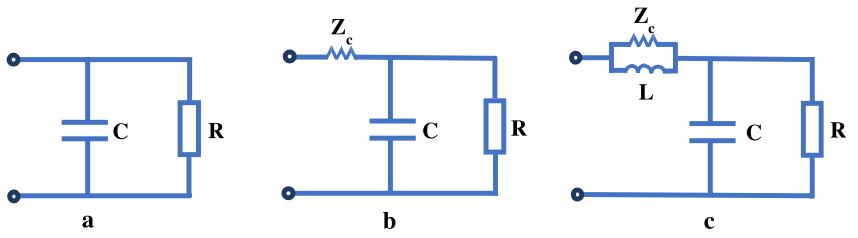
\includegraphics[width=\textwidth]{Figures/WK.JPG}
  \caption{Windkessel models \textbf{a} two-element; \textbf{b} three-element; \textbf{c} four-element \cite{Zhou2019APressure}}
  \label{fig:wind}
\end{figure}

To account for the interaction of the cardiac stroke volume with the compliance of the vessel, an electronic analogous model has been introduced at the outlets, a Windkessel model (different types shown in Figure \ref{fig:wind}). Three-element Windkessel (WK3) model is often used theoretical research. The circuit diagram of the model can be seen on Figure \ref{fig:0d}. \par

\begin{figure}[ht!]
  \centering
  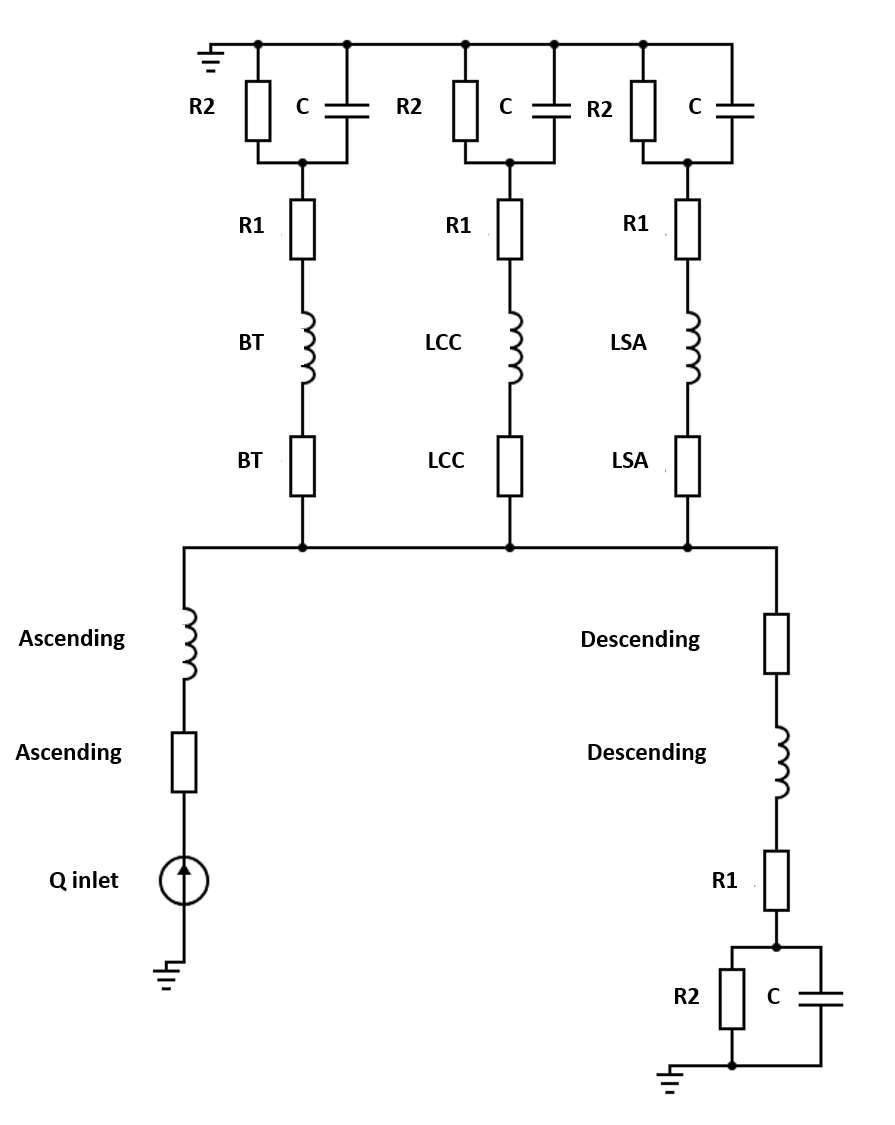
\includegraphics[width=0.5\textwidth]{Figures/circuit.png}
  \caption{Schematic of the 0D model of the aorta}
  \label{fig:0d}
\end{figure}


\subsection{Parameter tuning}
In order to get accurate patient-specific parameters for the given pressure measurements and flow rates, an optimization algorithm was used to tune the individual components of the WK3 at every outlet. \par

Initially, the whole system is described as a single WK3 model where the $R_1$ and $R_2$ have been set as a ratio $R_1/(R_1+R_2) = 5.6\%$ which simplifies the problem to only two parameters $R_1$ and $C$ that need to be fitted. The objective function minimizes the difference between the target systolic and diastolic pressure and the maximum and minimum pressure of the WK3 pressure curve which then gives:
\begin{align}
    min \sqrt{(P_{sys}-P_{max})^2+(P_{dia}-P_{min})^2}
\end{align}
 Additionally, non-negative constraints and bounding constraints have been applied for the parameters between the bounds [0, 2]. \par

Obtaining the parameters for the whole system, the total compliance is distributed proportionally to $\bar{Q_i}$ to the outlets and the resistances are set as a ratio as seen previously. Therefore, for the aorta, at each of the outlet, only one parameter needs to be optimized. The objective function sums up the difference in the target and model pulse pressure, and also the target and the model mean flow rate. As for the whole system model, non-negative constraints and bounding constraints were applied to the parameters. The objective function to be minimized is as following:
\begin{align}
    min \sqrt{(P_{sys}-P_{max})^2+(P_{dia}-P_{min})^2+\sum_{i}(\bar{Q}_{i}^{target}-\bar{Q}_{i}^{0D})^2}
\end{align}
The optimization method used to tune the parameter used was the Broyden–Fletcher–Goldfarb–Shanno algorithm.

\section{Boundary conditions}
The simulations were set up in ANSYS-CFX 19.0 (ANSYS Inc., PA, USA). The blood is modelled as incompressible with a density 1060 $kg m^{-3}$ and the flow was considered laminar, which is a common assumption in large arteries \cite{Alimohammadi2014DevelopmentConditions,Bonfanti2017ComputationalData}. The inlet condition was obtained from 4D-MRI and a flow rate was applied.\par

The three-element Windkessel parameters obtained from the 0D model were coupled to the outlet, relating the mean pressure (P) and the flow (Q) at the outlet via equation \ref{eq:PQ}
\begin{align}
    P=(R_1+R_2)Q-R_2C\frac{dP}{dt}+R_1R_2C\frac{dQ}{dt}
    \label{eq:PQ}
\end{align}
where $R_1$, $R_2$ and $C$ are the parameters obtained for each of the outlet. \par

A no-slip condition was applied, and the wall was considered as rigid. \par

\section{Modelling assumptions}
Different modelling assumptions can be used while modelling a patient aorta. The choice is often justified by the modeler but the resulting simulations can yield significantly different results. In this section, different modelling assumptions that were taken into account are discussed.

\subsection{Segmentation}
While the patient geometries were obtained from the images, the segmentation criterion can affect the resulting geometry primarily affecting the lumen's area. \par

To account for variation in the segmentation, two additional geometries were used, where the patient's aorta was dilated by 0.6 mm creating an expanded and narrow geometry. The amount of variation was based on the voxel size (1 mm) from which the aorta was segmented. \par

\subsection{Image processing}
Depending on the image processing choices and algorithm, smoothing can be applied to the segmentation of the aorta to account for the artefacts in the patient scans. \par

In the simulations two different aortas are being used, where one surface is smooth and the other is unsmooth as seen on the Figure \ref{fig:geometry}.

\begin{figure}[ht!]
    \centering
    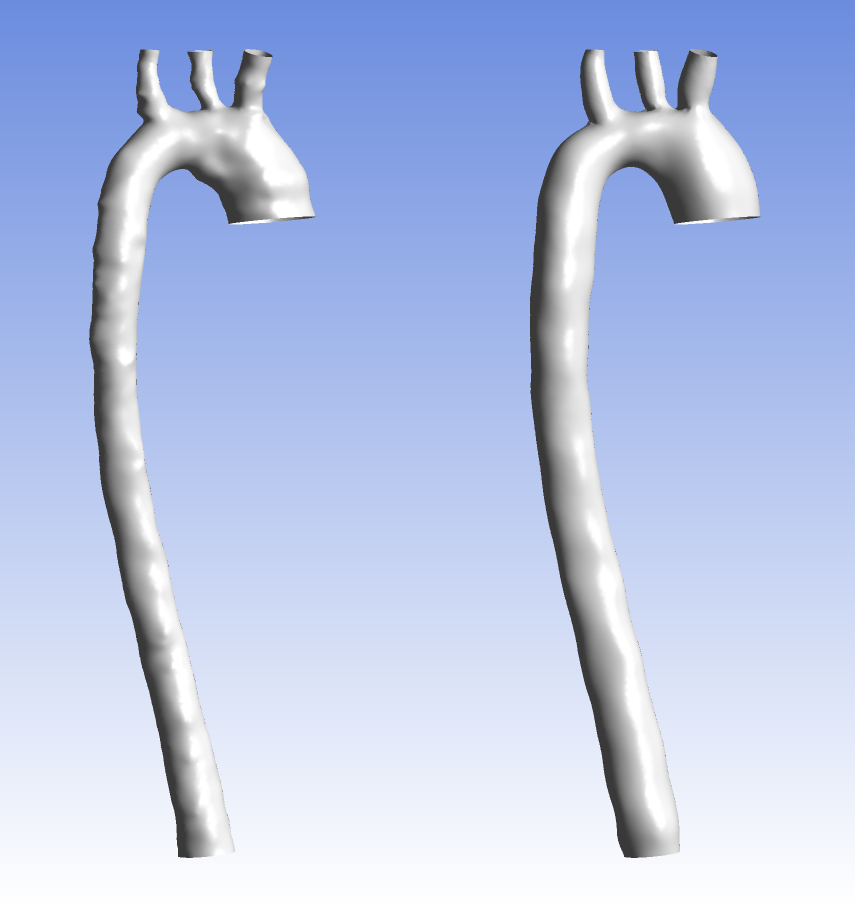
\includegraphics[width=0.5\textwidth]{Figures/Geometry.png}
    \caption{Unsmooth geometry (left) and smooth geometry (right used in the study which can be a result of decisions made during image processing}
    \label{fig:geometry}
\end{figure}

\subsection{Mesh}
While a finer mesh can yield much more accurate results, it comes with a trade-off of computational run time. In CFD simulations, it is  good practice to run mesh sensitivity studies before running the full simulation, however the decision on the mesh quality and approriateness is often left to the modeler.\par

In this project a several meshes were used to  assess how much the mesh can influence the final results. Four different meshes have been used with ~120,000 ~250,000, ~600,000, and ~1,100.000 elements (through this report, the different mesh models will be referred to as Mesh 1-4 models, where Mesh 1 is the coarsest mesh and Mesh 4 is the finest). All meshes were created in ANSYS Fluent (ANSYS Inc., PA, USA). \par

\subsection{Viscosity}
As seen in the Chapter \ref{chapterlabel2}, while blood has shearing properties it is often assumed as Newtonian in larger arteries. Another commonly used approximation, often used in simulations is the Carreau-Yasuda model to model non-Newtonian behaviour. \par

For this work, two blood models have been considered, a Newtonian model with a constant viscosity of 0.004 $Pa$ $s$ and a non-Newtonian model was modelled via the Carreau-Yasuda model, with the parameters taken from the Gijsen et al \cite{Gijsen1999TheModel}.

\section{Conceptual framework to assess structural uncertainty}
The conceptual framework uses permutations of assumptions to build additional models to analyse the uncertainty. By creating additional simulations, the variations across a number of simulation can be assess and the structural uncertainty can be addressed. In addition, study the variability of individual assumptions, it will be possible to evaluate the interacting error due to several assumptions.  \par

By combining the assumptions mentioned above, the framework for a single patient results in 48 different CFD models. \par


\section{Numerical simulations and post-processing}
The simulations run until reaching the periodic steady-state, which was achieved after running three cardiac cycles. For the analysis, the last cycle was used for analysis of the flow and calculation of the time-averaged wall shear stress (TAWSS). 

\begin{equation}
TAWSS=\frac{1}{T}\int_{0}^{T} |\tau(t)|dt
\label{eq:tawss}
\end{equation}
where $|\tau(t)|$ is the magnitude of WSS at the time $t$. \par

The post-processing was done in CFD-Post (ANSYS Inc., PA, USA) and by Python (Python Software Foundation, DE, USA).


\chapter{Results}
\label{chapterlabel6}

A "control simulation" will be defined as the case that is most commonly used in literature. The case used as control will be a normal-sized aorta, smooth wall and Newtonian fluid. The mesh selected was mesh 3 ($\sim$600,000 elements) \cite{Steinman2012AssumptionsHemodynamics}.

\section{Outlet flow and pressure comparison}
A comparison of the outlet conditions was performed. The results were compared by calculating the mean absolute percentage error (MAPE) between control model and the model with modified assumptions:

\begin{align}
    MAPE =| \frac{y_{i}-y_{control}}{y_{control}}| \times 100 \%
\end{align}

where y is the parameter of interest, which in this comparison would be either the flow rate or the pressure. \par
A comparison of the outlet pressure and flow can be seen on the Figures \ref{fig:flow} and \ref{fig:pressure}. A comparison with the control simulation shows that the pressure at the outlets are very similar across the models as the mean absolute percentage error is less then 1\% (as seen in the Table \ref{tab:pererr}). However, significant differences can be seen in the flow curves, depending on the model assumptions taken into account. On the Table \ref{tab:pererr}, very small differences can be seen when the viscosity model is modified while the dilation of the aortic geometry results in a much larger MAPE.
\begin{figure}
     \centering
     \begin{subfigure}[b]{0.49\textwidth}
         \centering
         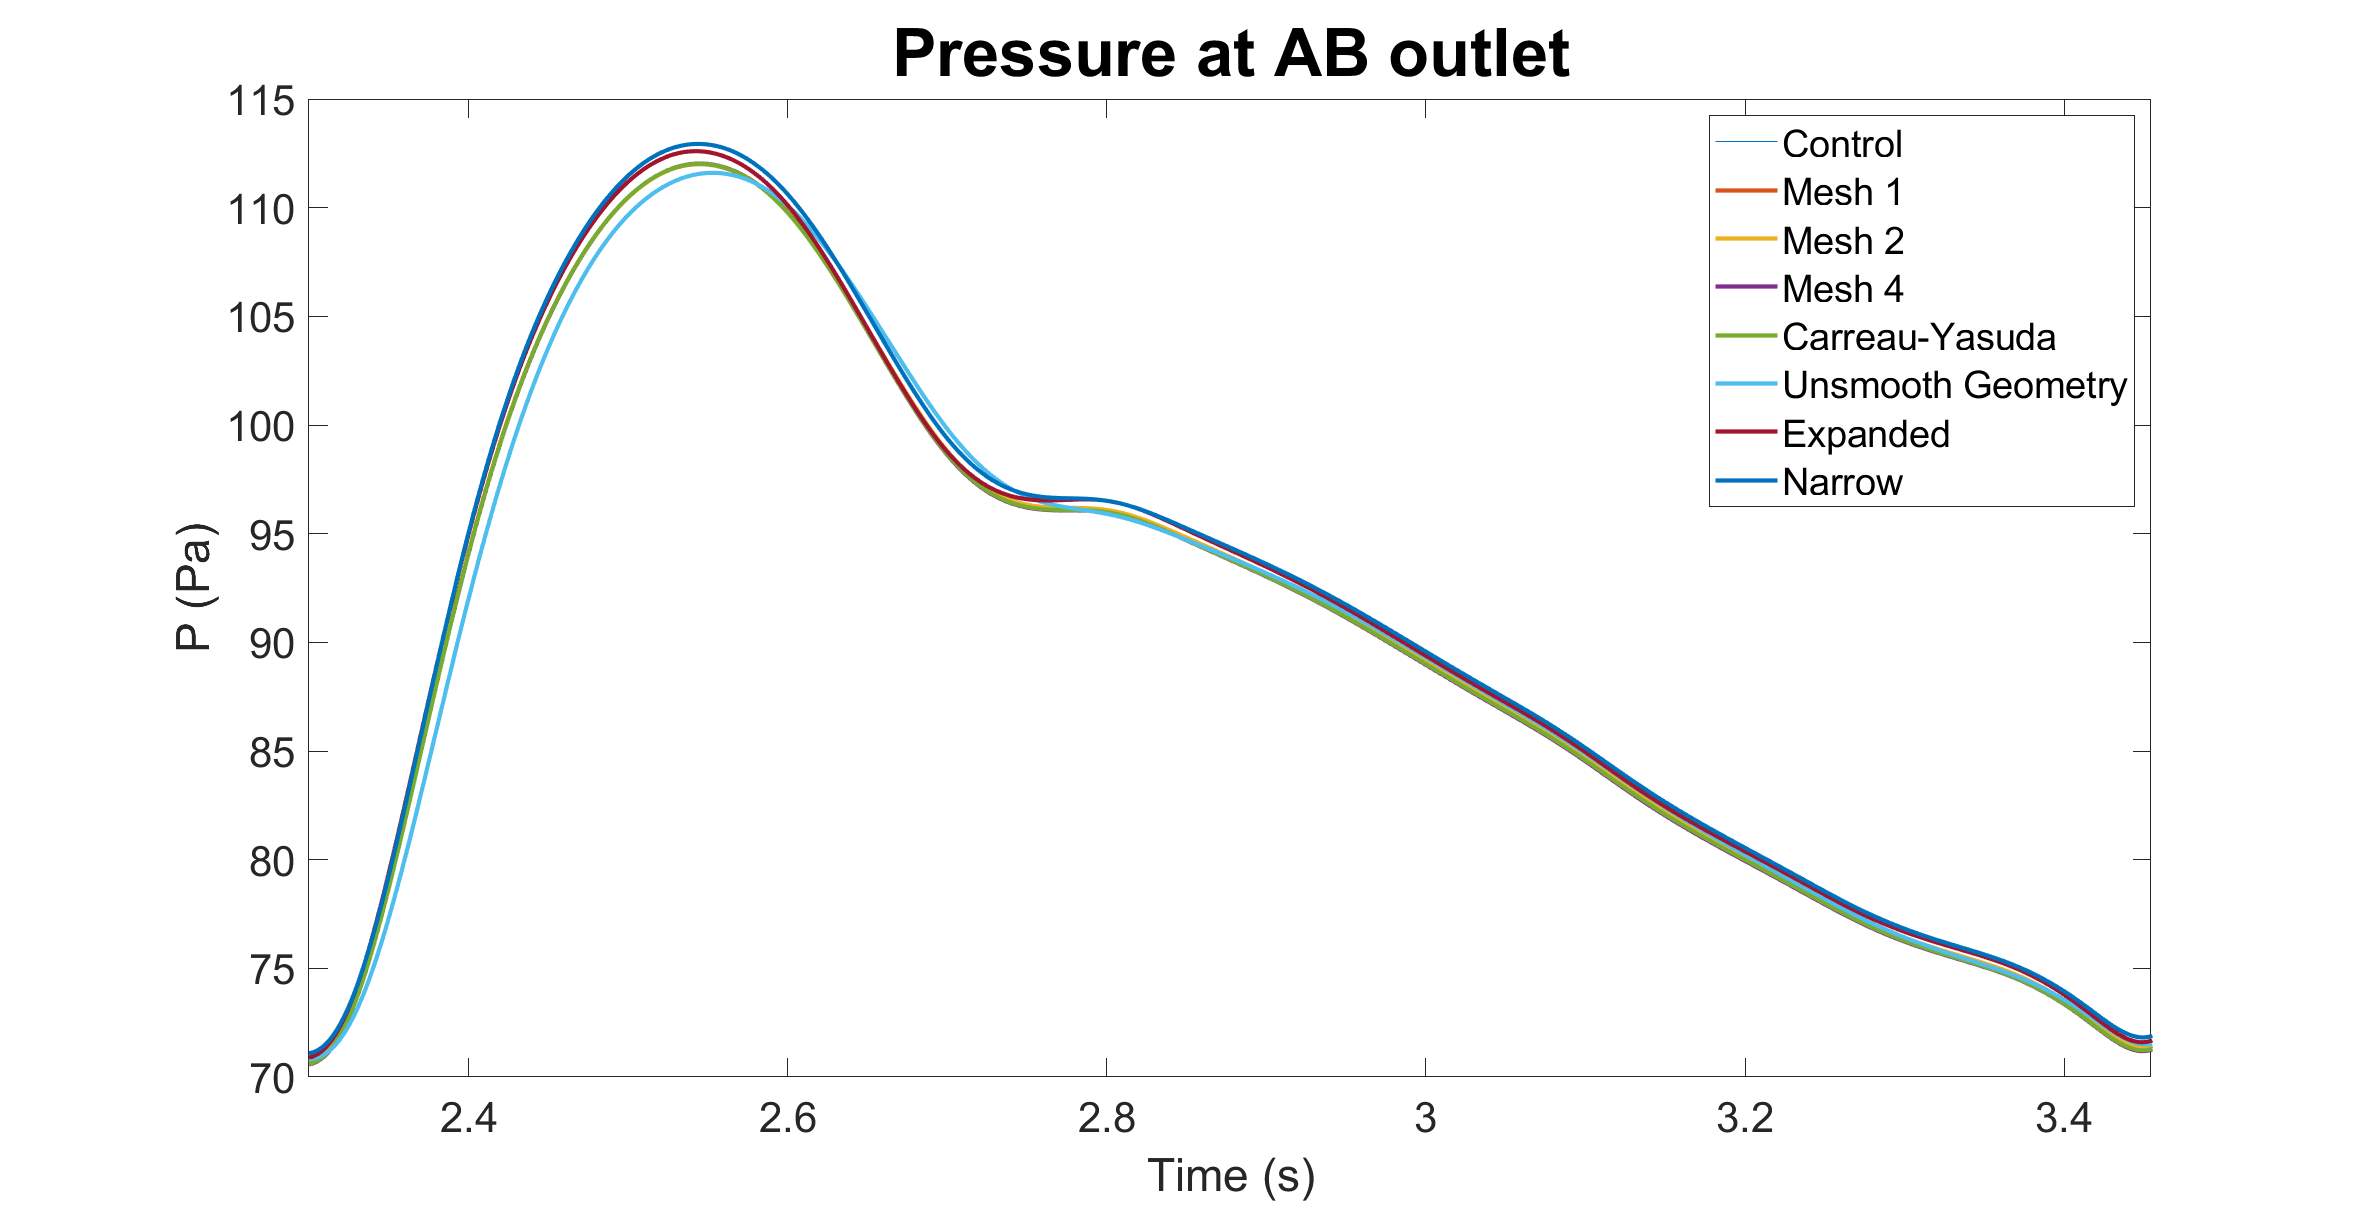
\includegraphics[width=\textwidth]{Figures/PAB.png}
     \end{subfigure}
     \hfill
     \begin{subfigure}[b]{0.49\textwidth}
         \centering
         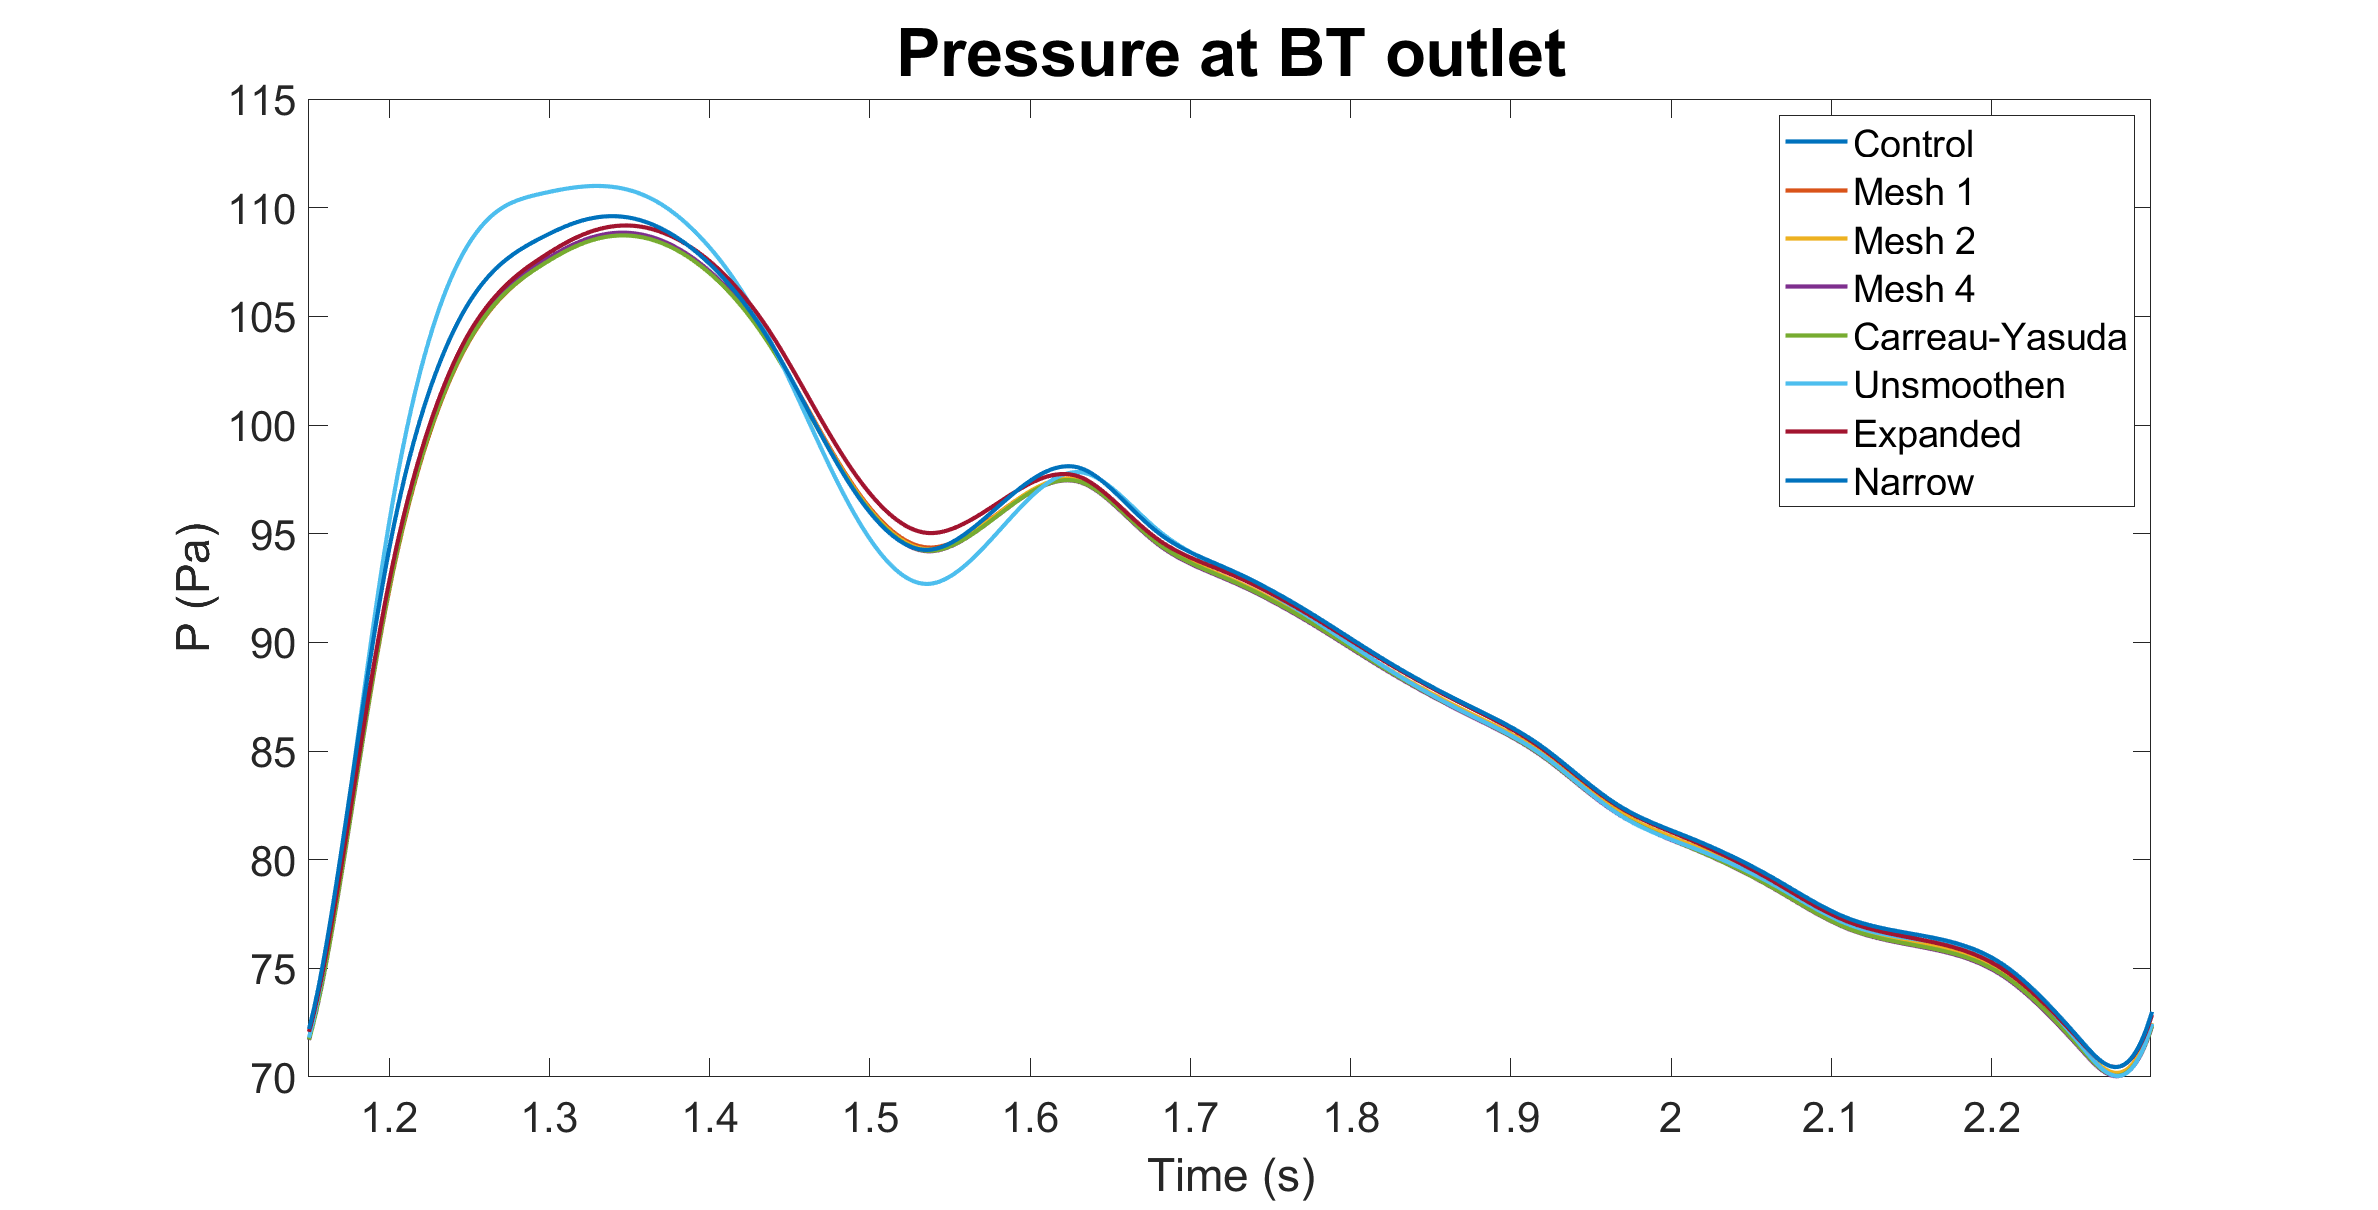
\includegraphics[width=\textwidth]{Figures/PBT.png}
     \end{subfigure}
     \hfill
     \begin{subfigure}[b]{0.49\textwidth}
         \centering
         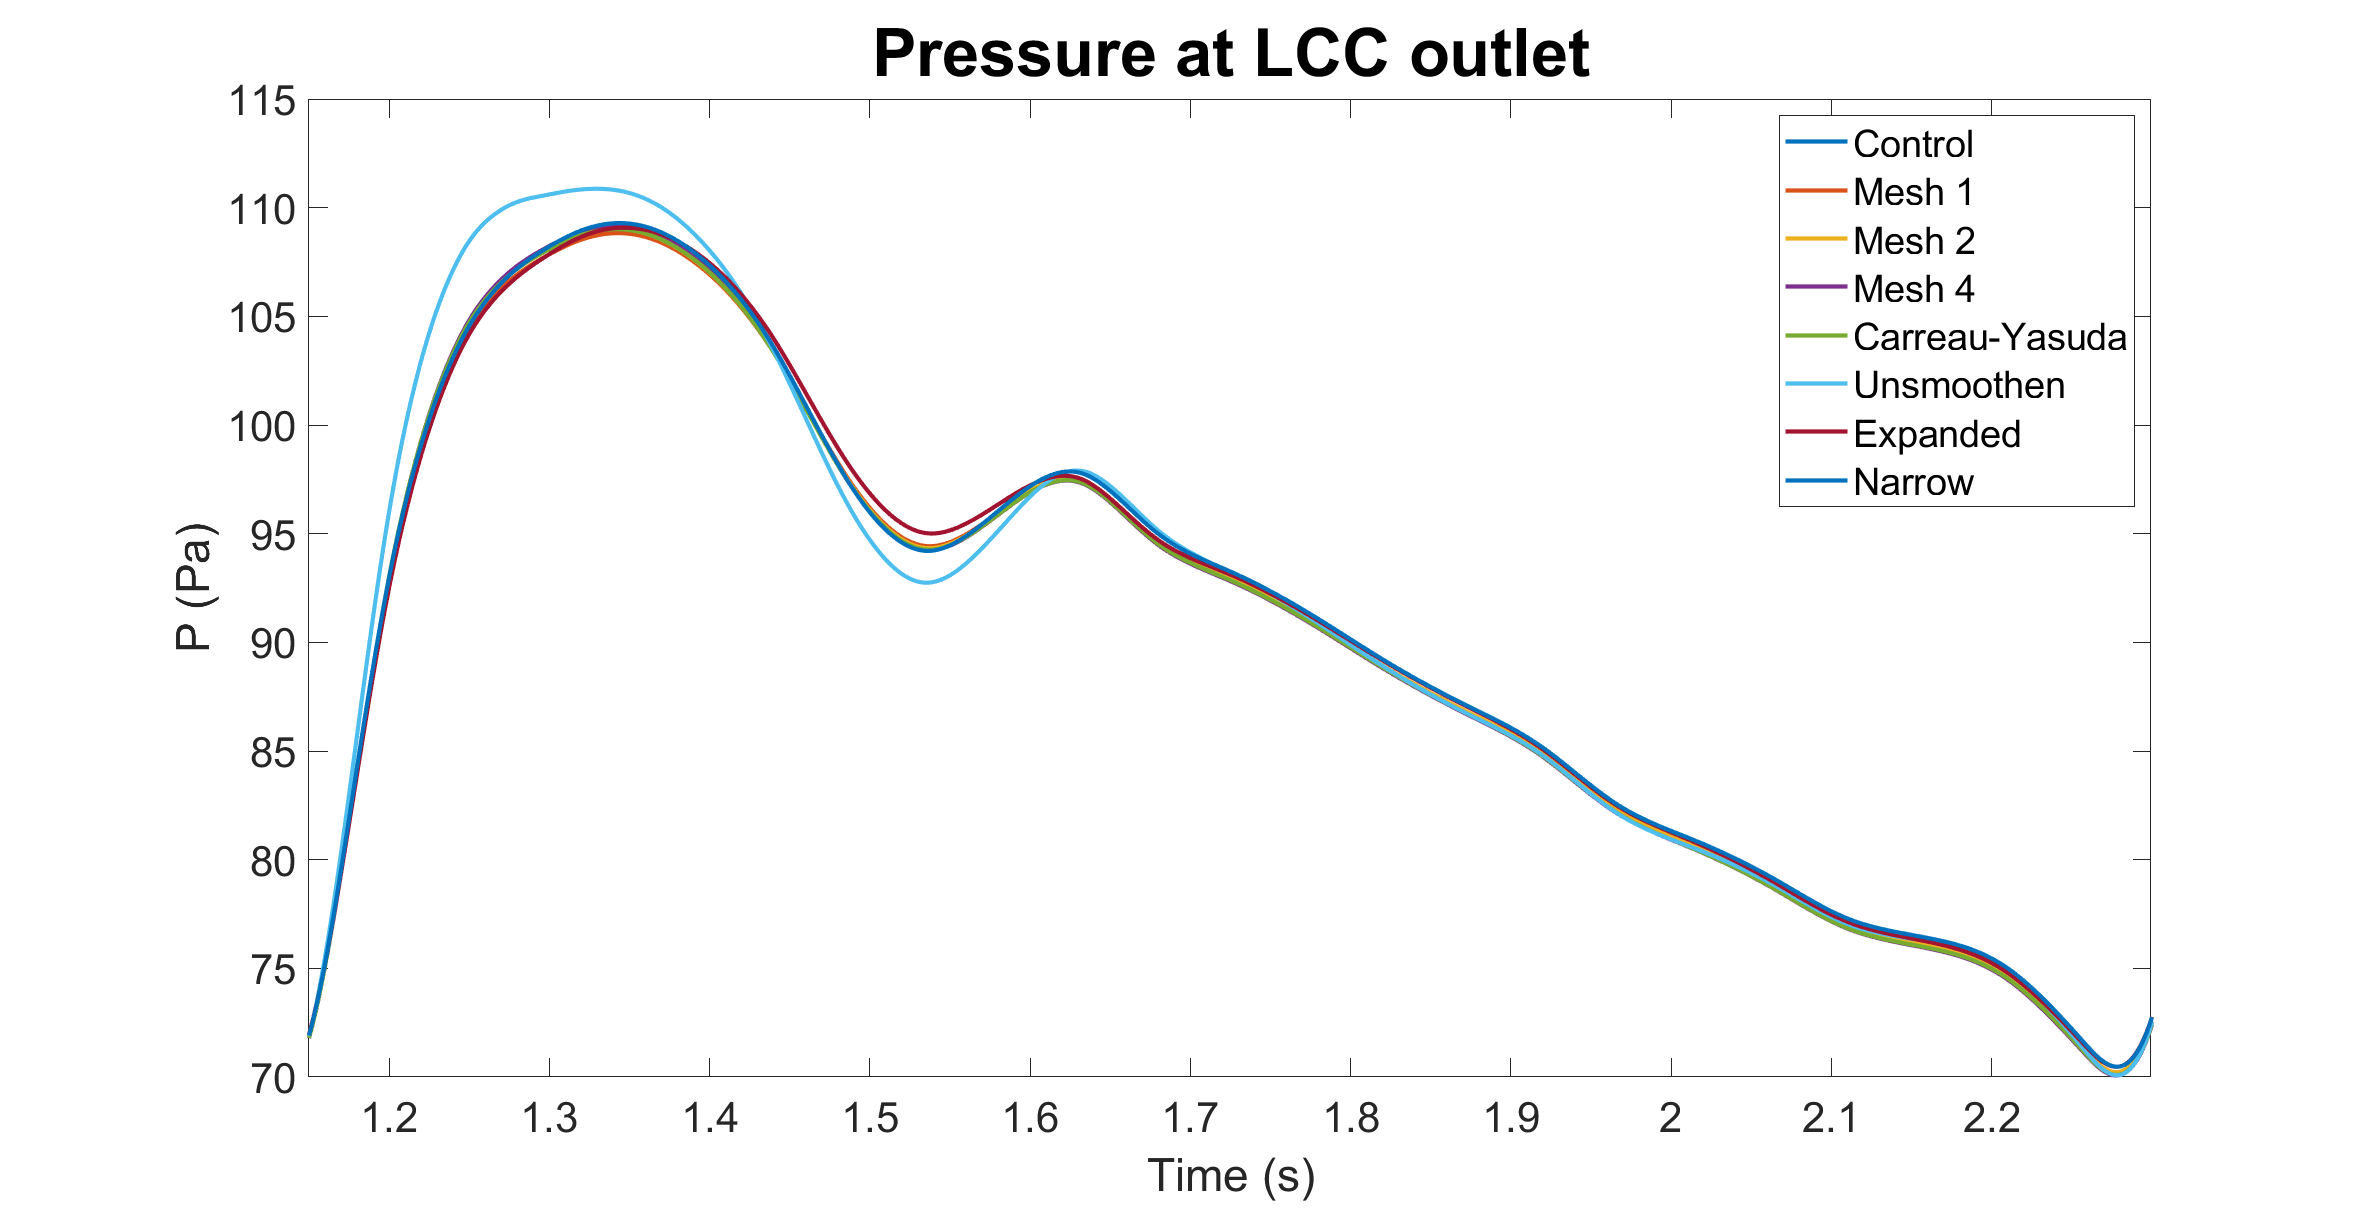
\includegraphics[width=\textwidth]{Figures/PLCC.png}
     \end{subfigure}
     \hfill
     \begin{subfigure}[b]{0.49\textwidth}
         \centering
         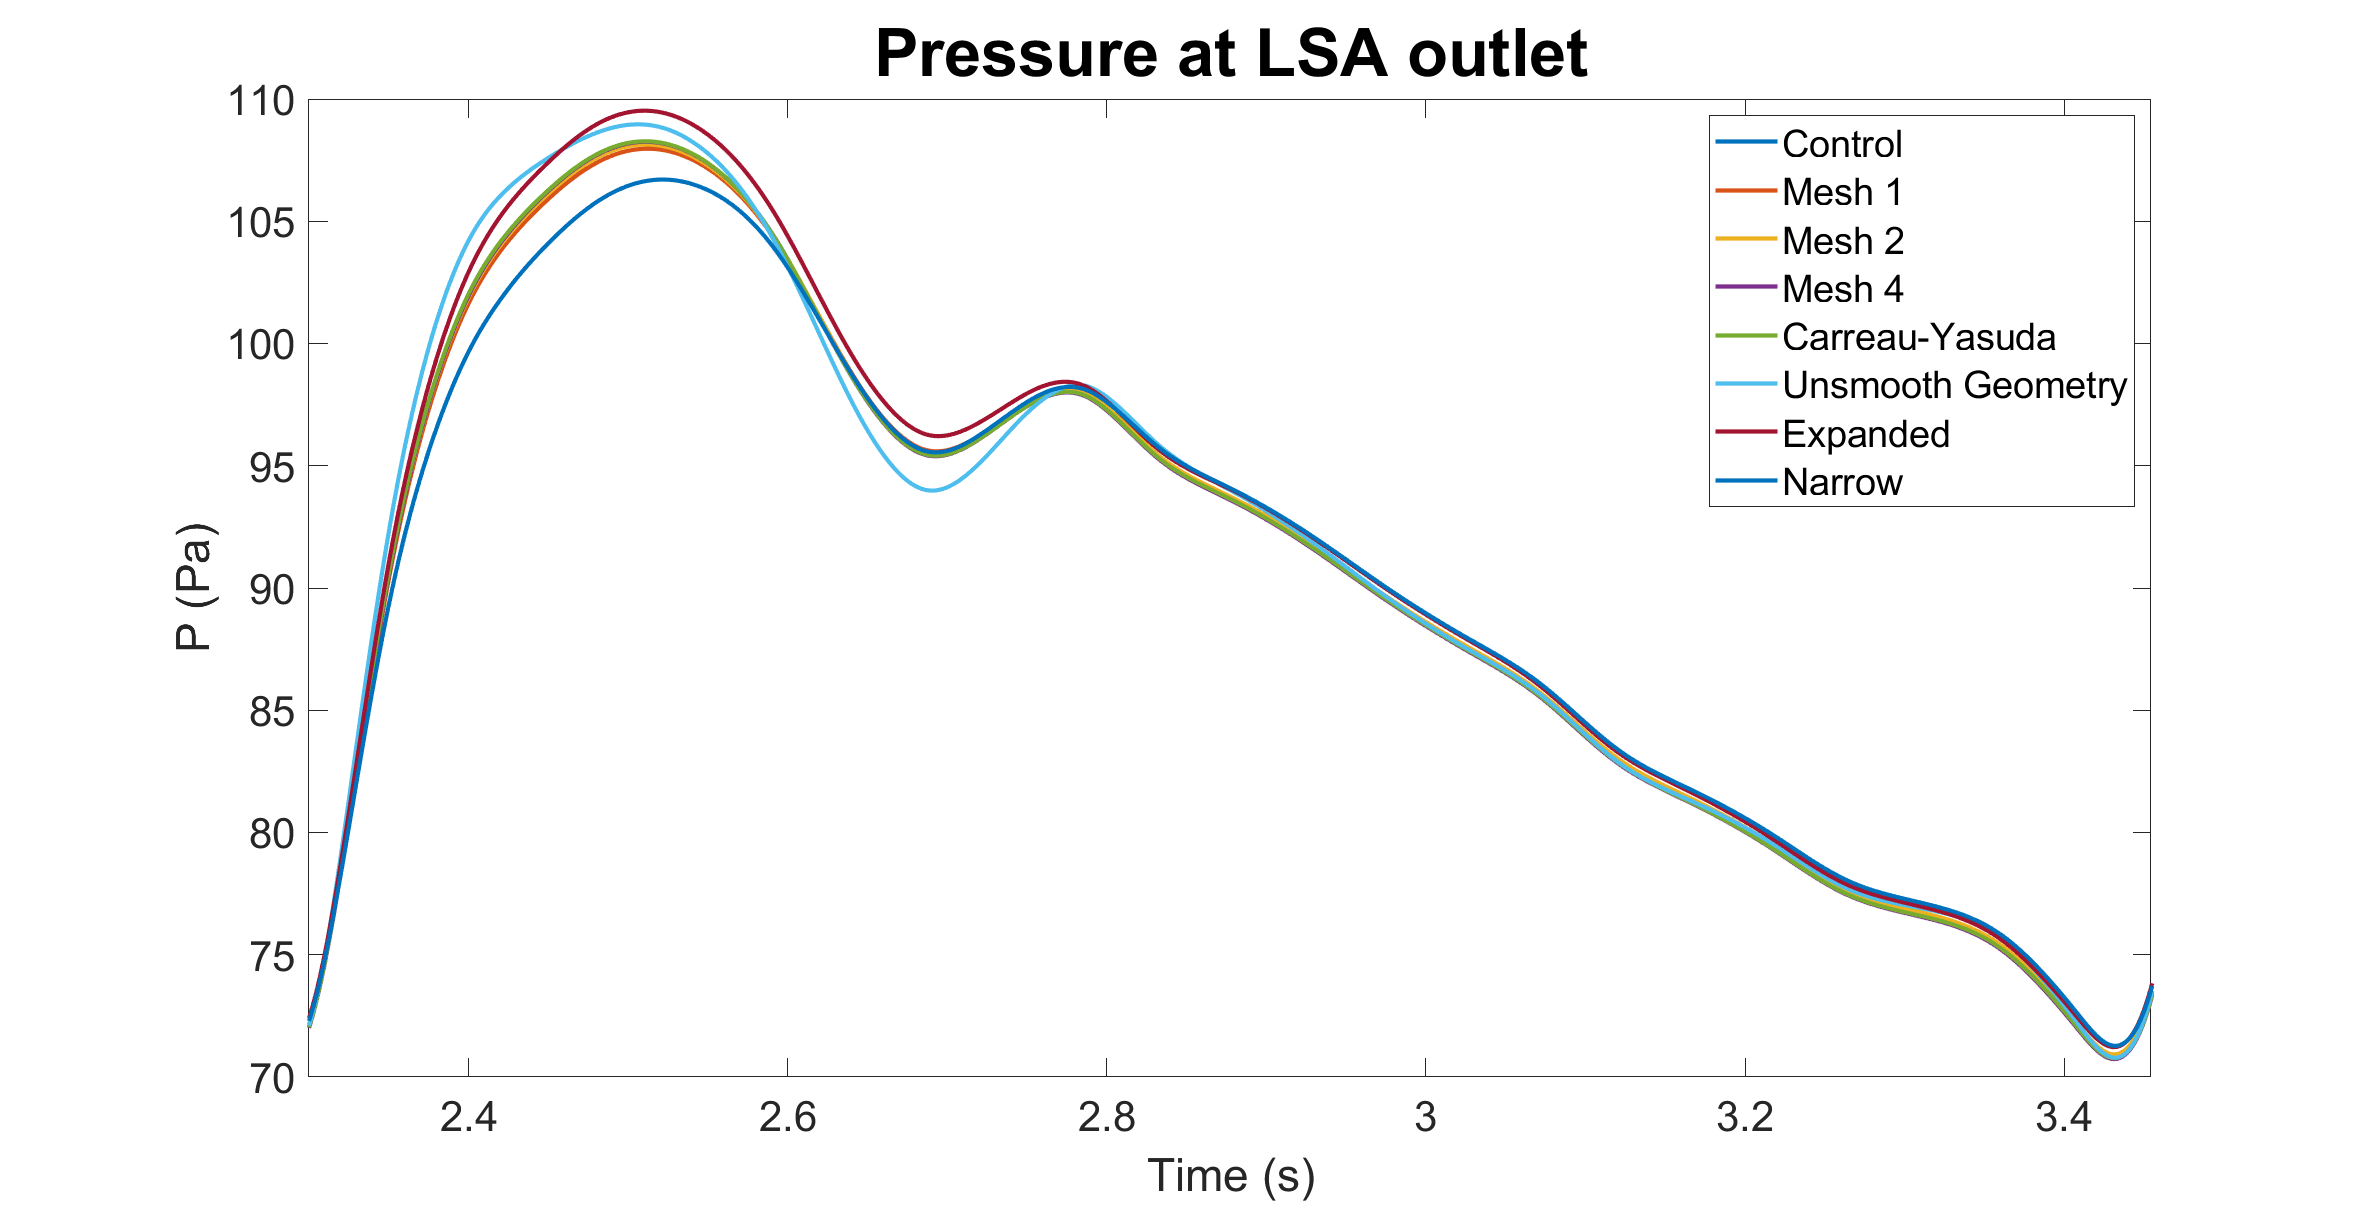
\includegraphics[width=\textwidth]{Figures/PLSA.png}
     \end{subfigure}
        \caption{The pressure at the different outlets}
        \label{fig:pressure}
\end{figure}

\begin{figure}
     \centering
     \begin{subfigure}[b]{0.49\textwidth}
         \centering
         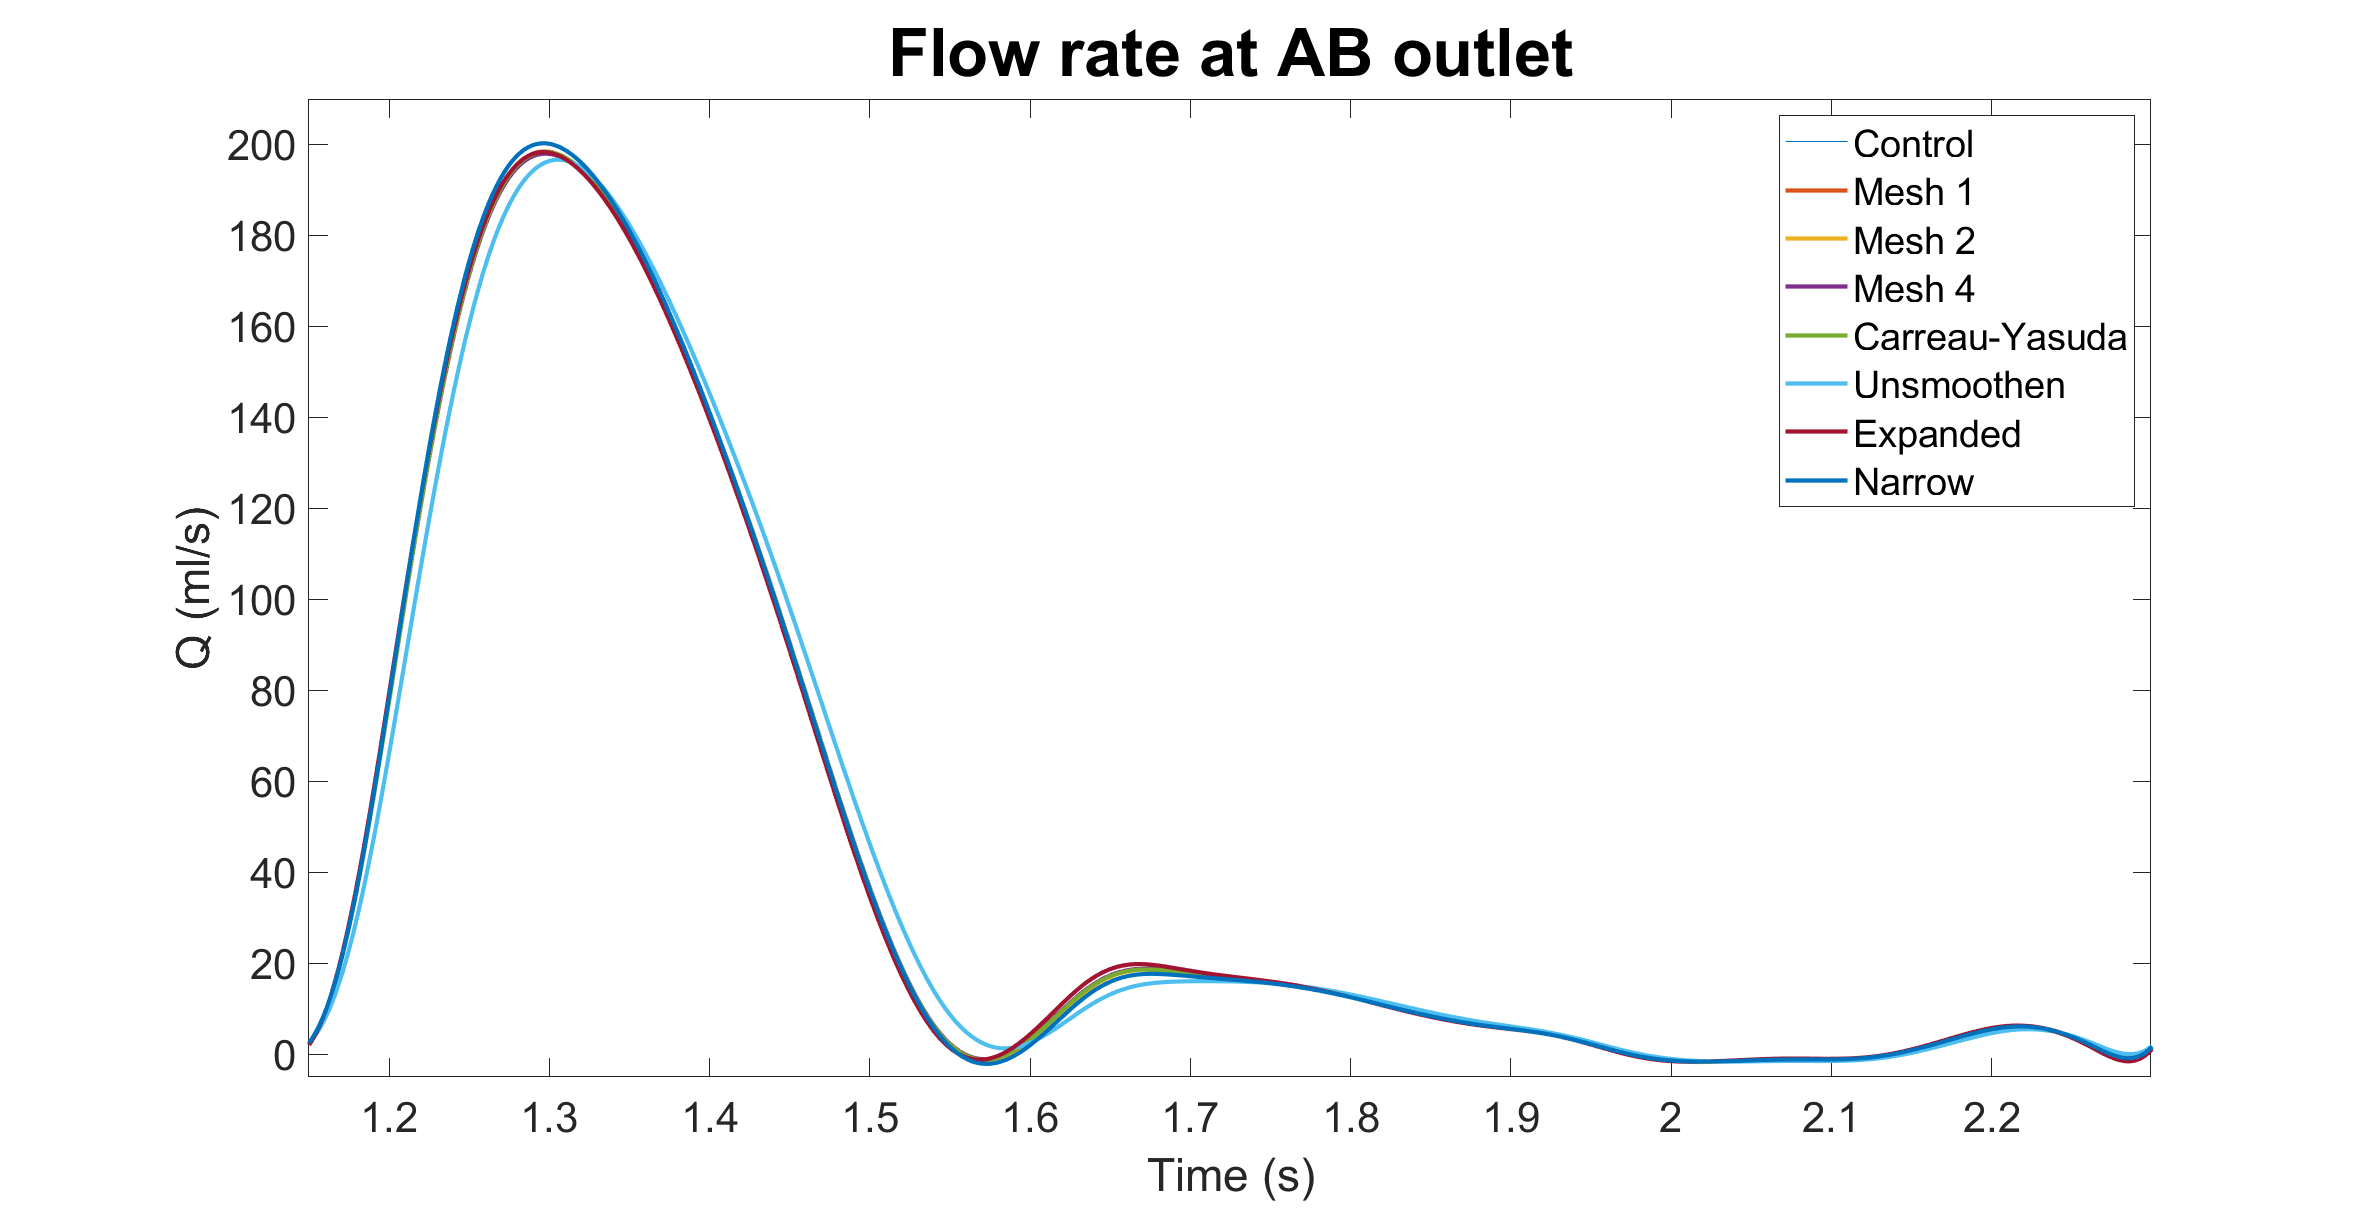
\includegraphics[width=\textwidth]{Figures/QAB.png}
     \end{subfigure}
     \hfill
     \begin{subfigure}[b]{0.49\textwidth}
         \centering
         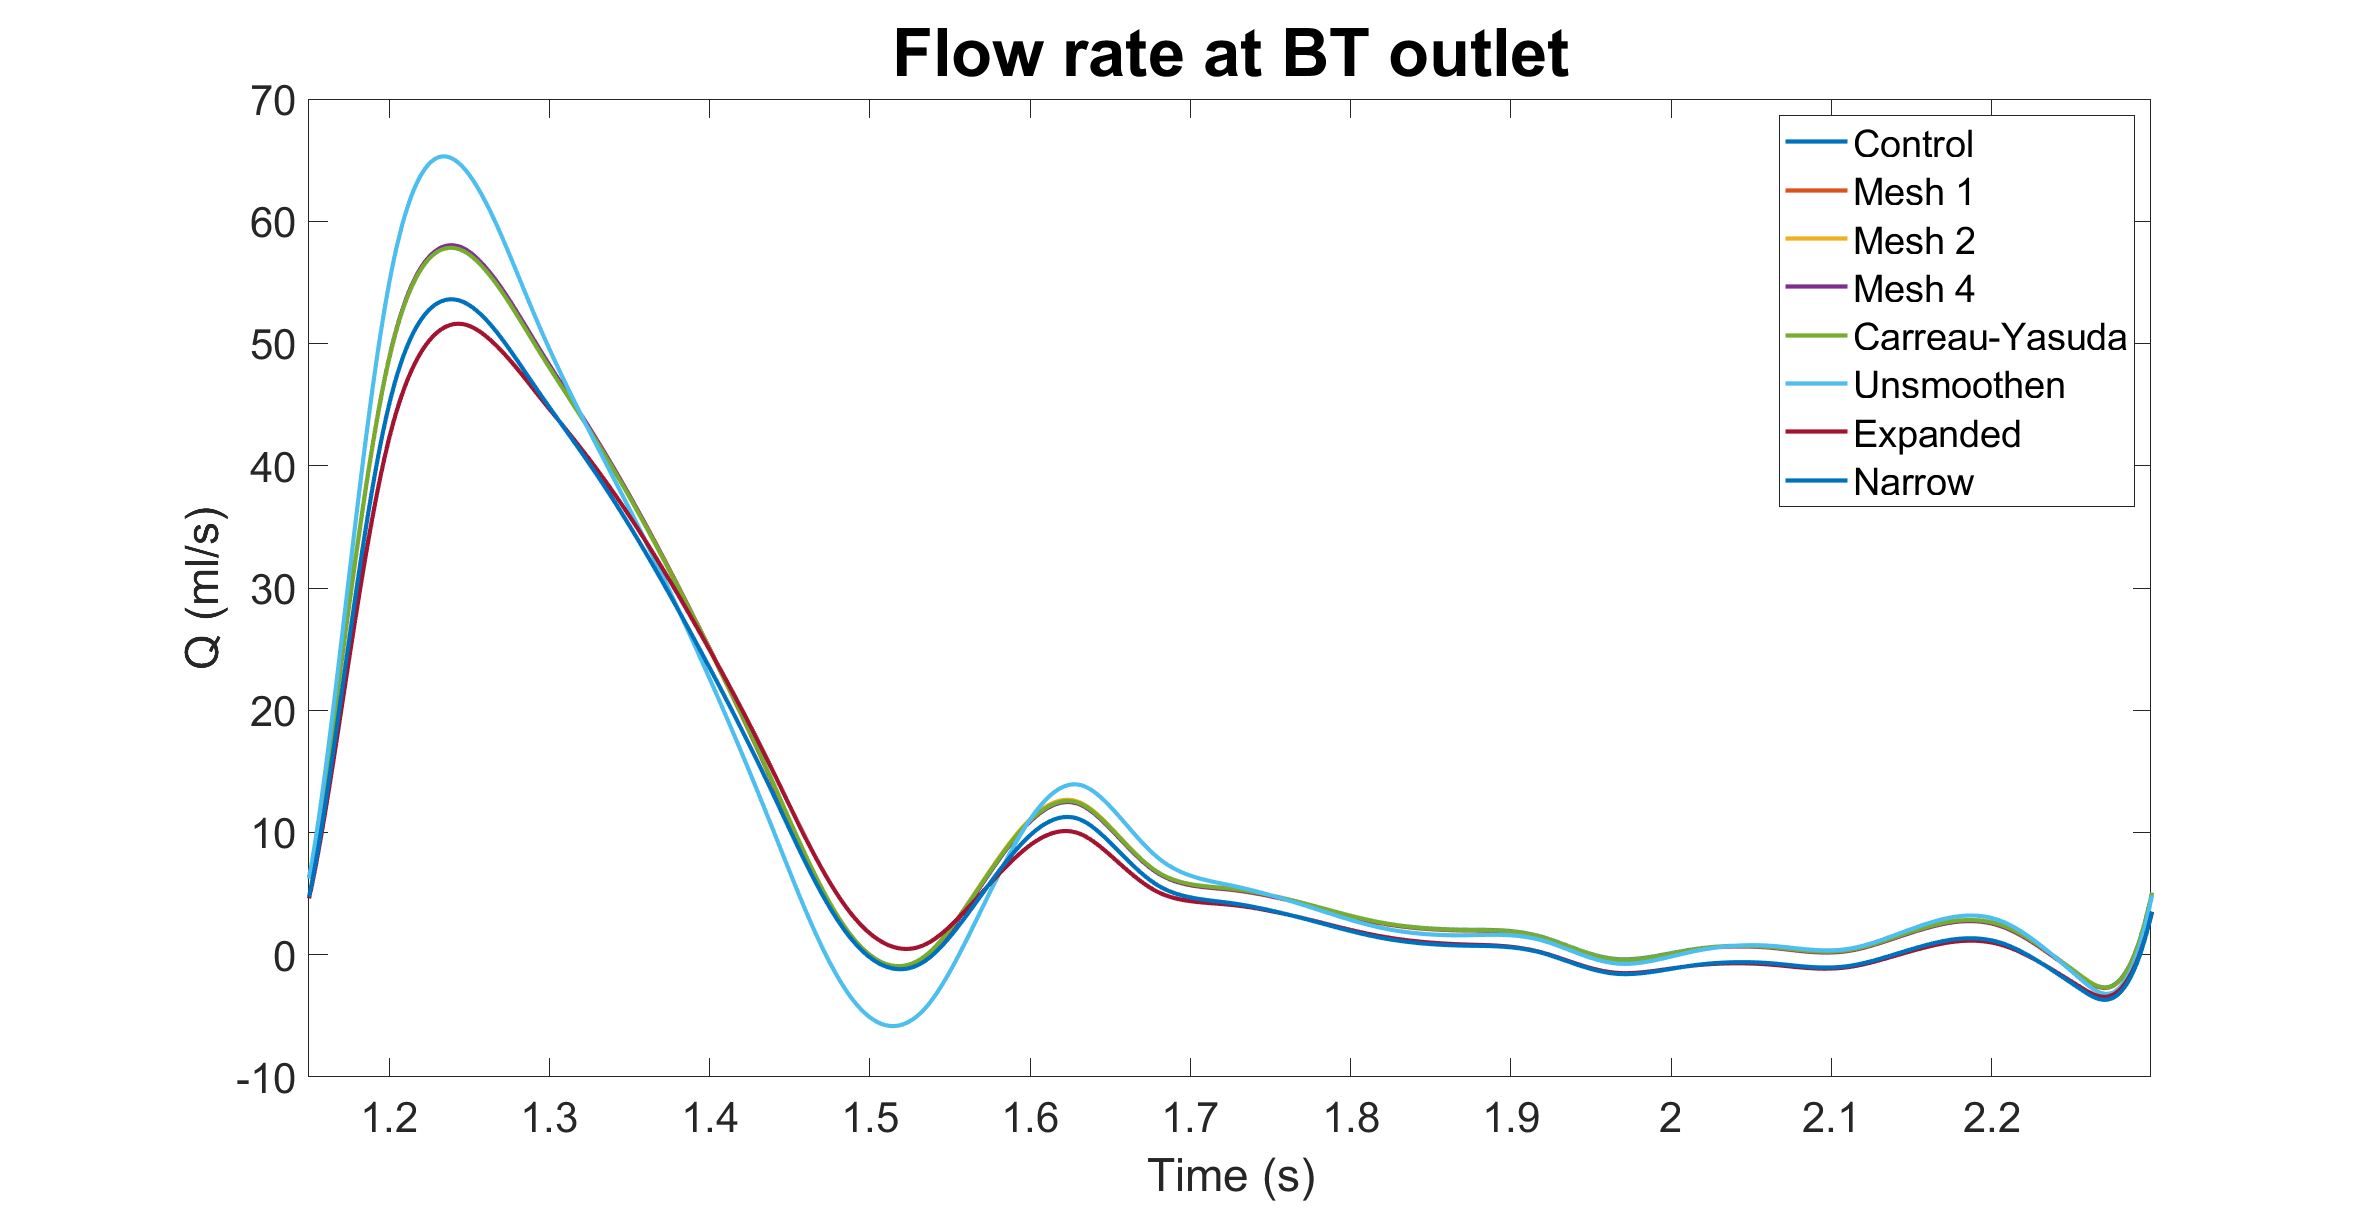
\includegraphics[width=\textwidth]{Figures/QBT.png}
     \end{subfigure}
     \hfill
     \begin{subfigure}[b]{0.49\textwidth}
         \centering
         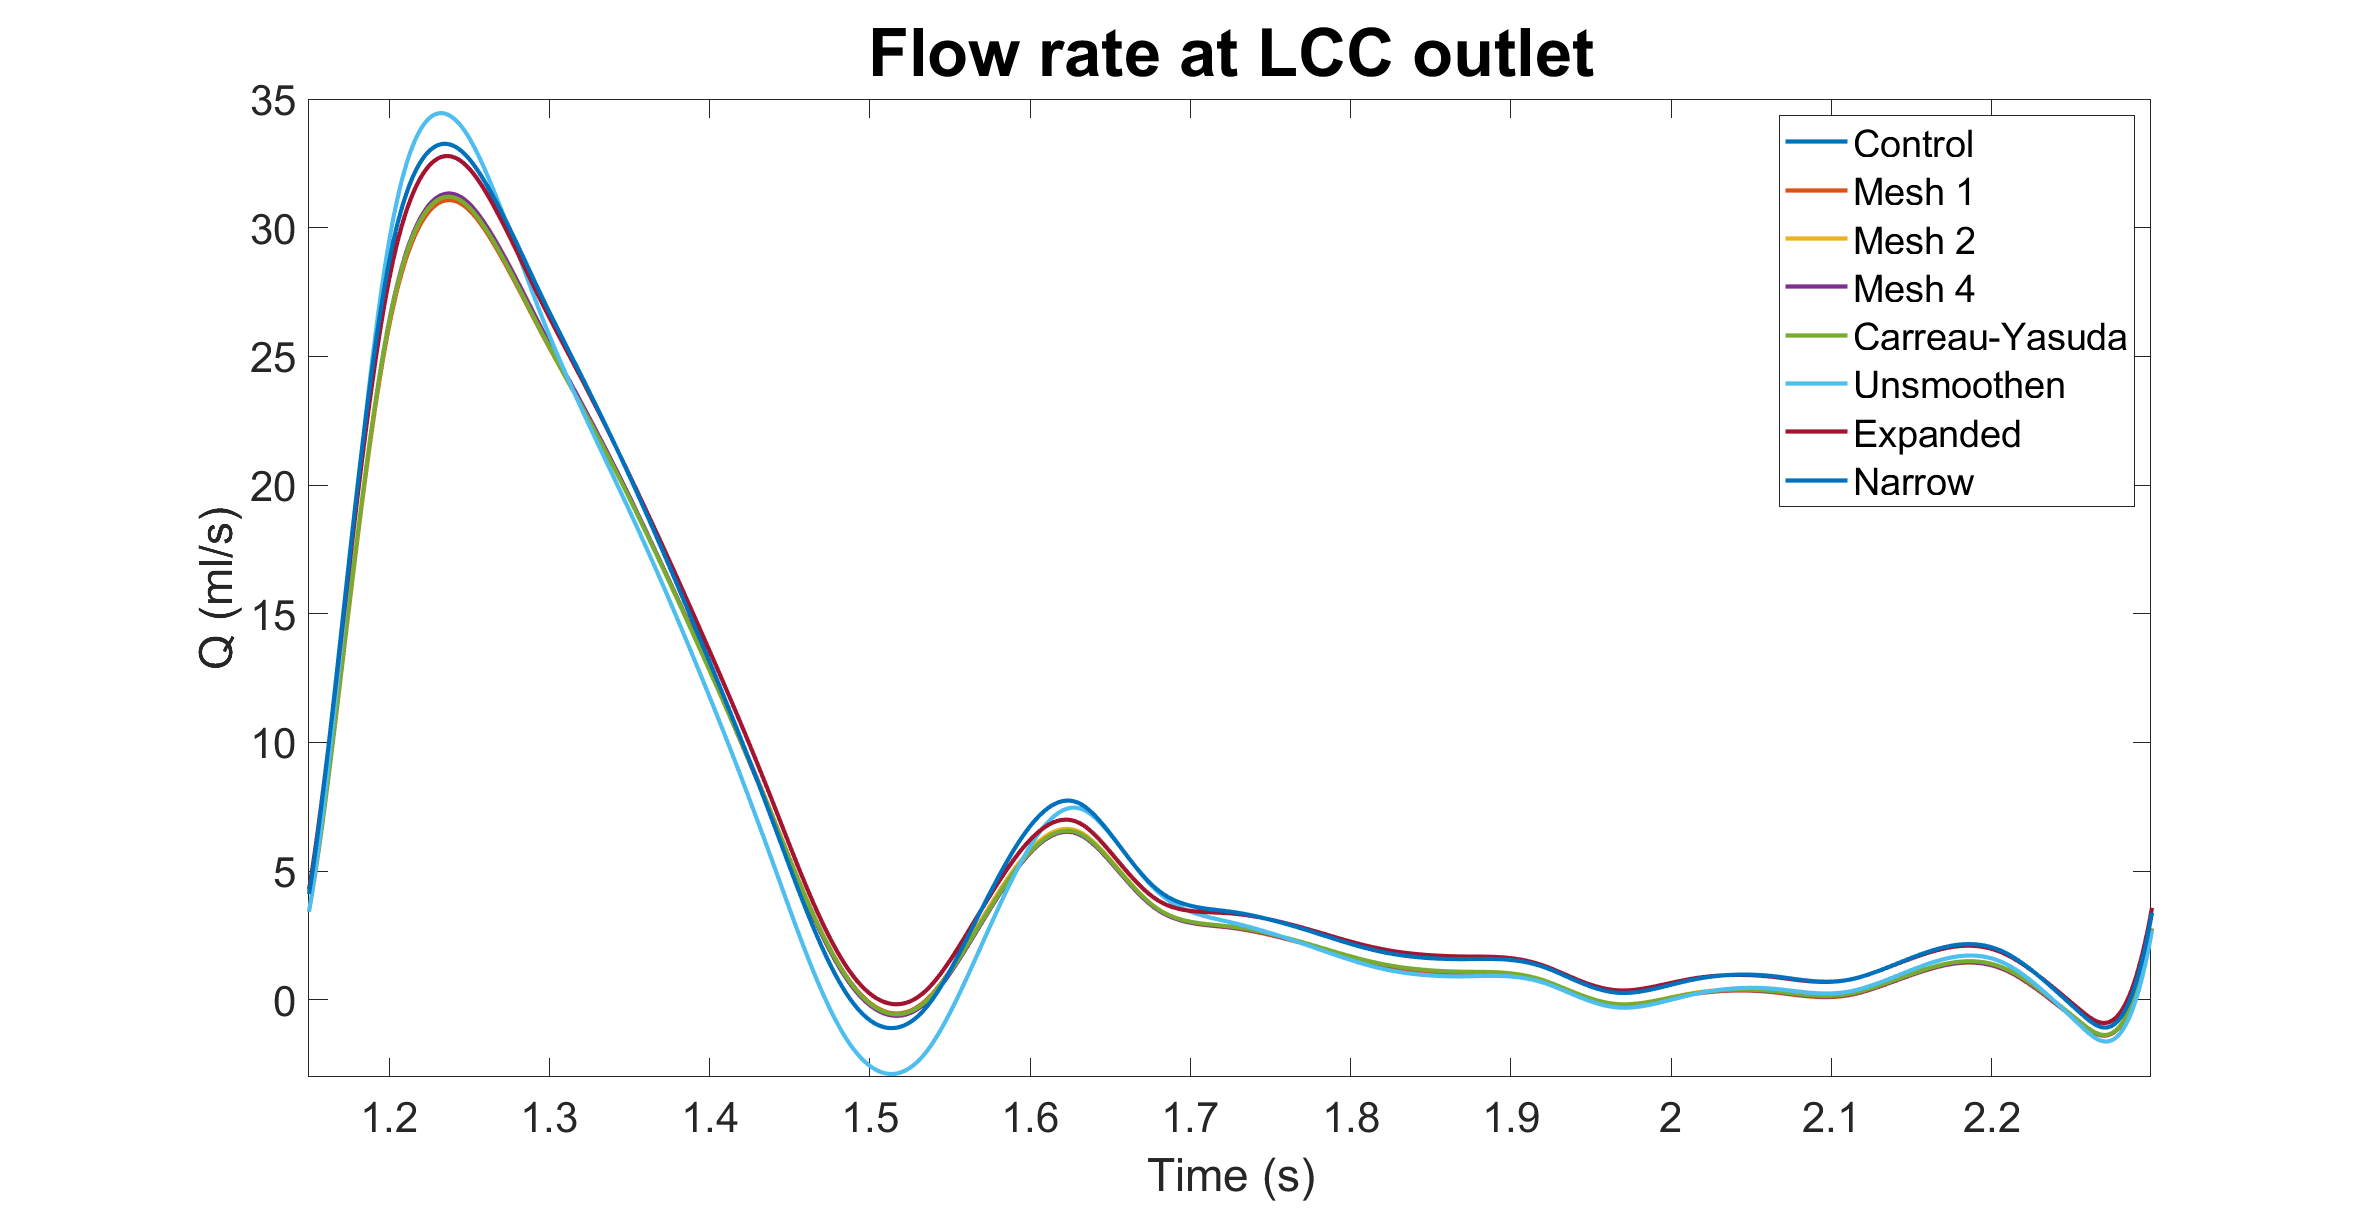
\includegraphics[width=\textwidth]{Figures/QLCC.png}
     \end{subfigure}
     \hfill
     \begin{subfigure}[b]{0.49\textwidth}
         \centering
         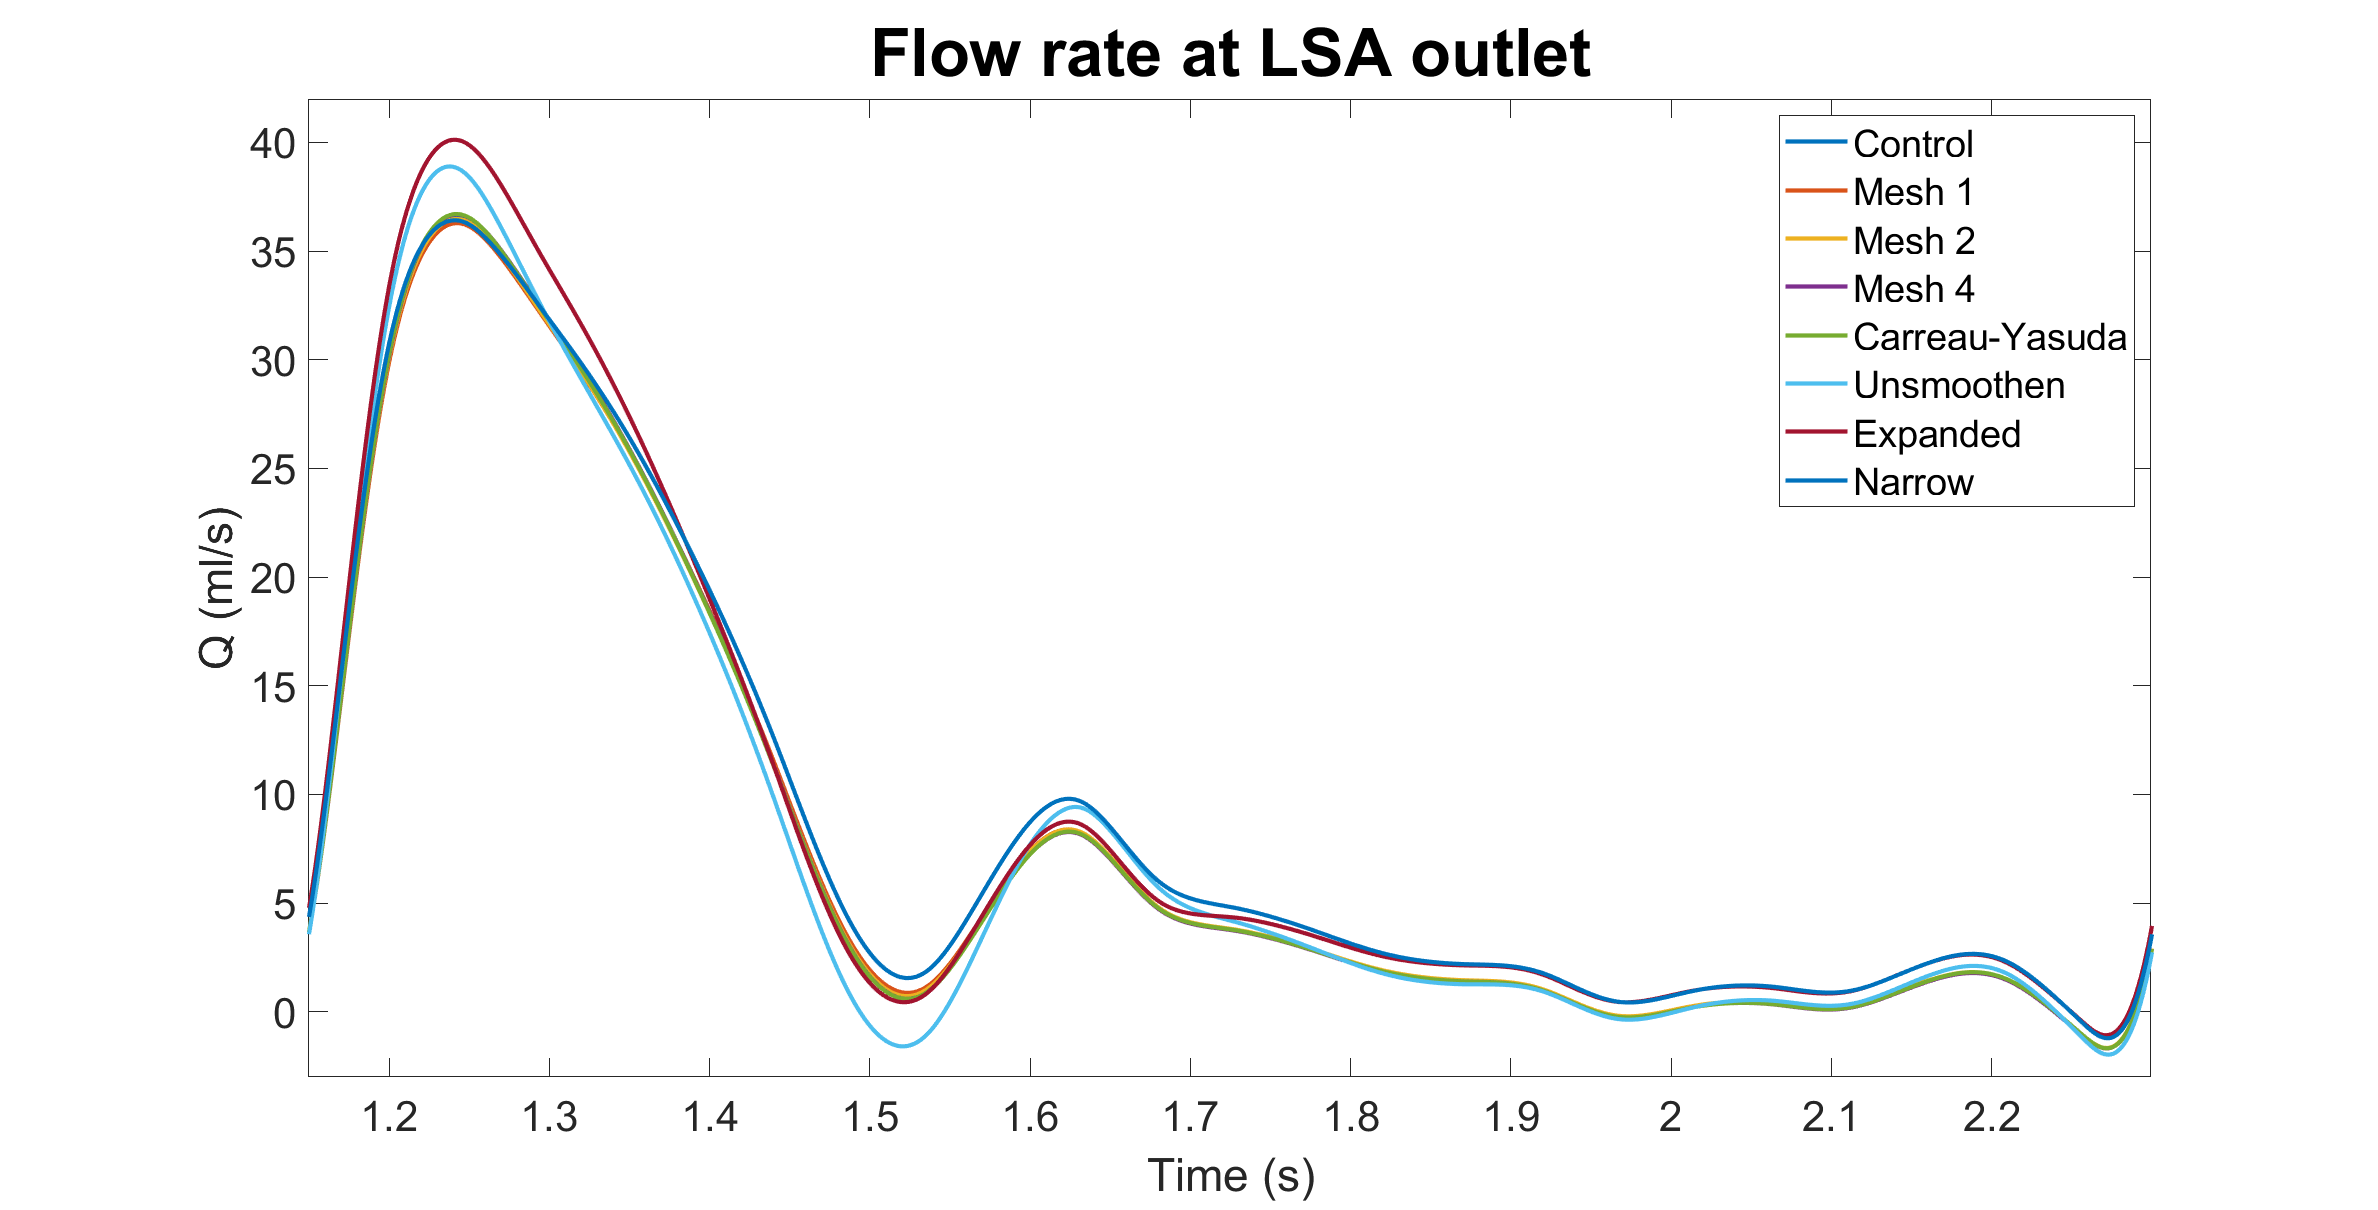
\includegraphics[width=\textwidth]{Figures/QLSA.png}
     \end{subfigure}
        \caption{The flow at the different outlets}
        \label{fig:flow}
\end{figure}

The most noticeable differences can be observed on the dilated geometries of the patient aorta, where the MAPE of the flow was up to  245.78\% at one of the outlet followed by the image processing influence, where the difference was 270.79\%. The smallest difference was shown to be the influence of the viscosity model, where the maximum MAPE is 6.24\%. The influence of the mesh showed varying results where the highest MAPE was calculated on the Mesh 1 with the maximum difference of 18.69\%. \par

\begin{table}[ht!]
\resizebox{\textwidth}{!}{%
\begin{tabular}{l|ccccccccc}
 & \multicolumn{9}{c}{Mean absolute percentage error (\%)} \\
Model & $P_{AB}$ & $P_{BT}$ & $P_{LCC}$ & $P_{LSA}$ & $P_{in}$ & $Q_{AB}$ & $Q_{BT}$ & $Q_{LCC}$ & $Q_{LSA}$ \\ \hline
Mesh 1 & 0.05 & 0.07 & 0.11 & 0.12 & 0.07 & 9.11 & 10.28 & 18.69 & 3.49 \\
Mesh 2 & 0.07 & 0.07 & 0.07 & 0.09 & 0.07 & 4.69 & 5.78 & 3.22 & 9.32 \\
Mesh 4 & 0.05 & 0.05 & 0.06 & 0.05 & 0.05 & 4.59 & 8.20 & 6.05 & 1.69 \\
Carreau-Yasuda & 0.03 & 0.04 & 0.04 & 0.04 & 0.06 & 3.11 & 6.24 & 4.27 & 3.63 \\
Unsmooth geometry & 0.51 & 0.85 & 0.76 & 0.53 & 1.00 & 71.36 & 270.79 & 138.30 & 36.97 \\
Expanded & 0.32 & 0.39 & 0.34 & 0.50 & 0.53 & 16.38 & 234.40 & 245.78 & 152.72 \\
Narrow & 0.52 & 0.56 & 0.35 & 0.69 & 0.77 & 18.40 & 180.13 & 224.91 & 159.92
\end{tabular}%
}
\caption{The mean absolute percentage error at the outlets between the different models and control}
\label{tab:pererr}
\end{table}

\section{Haemodynamic indices}
The results of TAWSS can be seen on the Table \ref{tab:meanTAWSS}. On the Figures \ref{fig:TAWSScontrol}-\ref{fig:TAWSSGeo1}, the aorta was divided in sections along the centerline and at every section, a box plot of haemodynamic indices was plotted. The box plot shows the mean of the values in the section with the red line, the $25^{th}$ and $75^{th}$ percentile of all the values and the maximum and the maximum the lines signify the maximum and minimum value. \par

\begin{table}[ht!]
\resizebox{\textwidth}{!}{%
\begin{tabular}{l|cccc}
 & \multicolumn{4}{c}{Mean TAWSS + SD at different locations (Pa)} \\
 & \multicolumn{1}{c|}{Ascending} & \multicolumn{1}{c|}{Arch} & \multicolumn{1}{c|}{Branches} & Descending \\ \hline
Control & \multicolumn{1}{c|}{0.996±0.630} & \multicolumn{1}{c|}{1.743±0.565} & \multicolumn{1}{c|}{1.979±0.893} & 1.152±0.388 \\
Mesh 1 & \multicolumn{1}{c|}{0.969±0.519} & \multicolumn{1}{c|}{1.714±0.543} & \multicolumn{1}{c|}{1.706±0.792} & 1.114±0.362 \\
Mesh 2 & \multicolumn{1}{c|}{0.986±0.562} & \multicolumn{1}{c|}{1.748±0.549} & \multicolumn{1}{c|}{1.832±0.829} & 1.154±0.390 \\
Mesh 4 & \multicolumn{1}{c|}{0.968±0.638} & \multicolumn{1}{c|}{1.708±0.556} & \multicolumn{1}{c|}{2.297±1.073} & 1.157±0.389 \\
CY & \multicolumn{1}{c|}{0.996±0.545} & \multicolumn{1}{c|}{1.633±0.478} & \multicolumn{1}{c|}{1.820±0.726} & 1.133±0.325 \\
Unsmooth geometry & \multicolumn{1}{c|}{1.357±0.798} & \multicolumn{1}{c|}{1.798±0.987} & \multicolumn{1}{c|}{2.468±1.522} & 1.757±0.852 \\
Expanded & \multicolumn{1}{c|}{0.938±0.545} & \multicolumn{1}{c|}{1.490±0.523} & \multicolumn{1}{c|}{1.498±0.700} & 1.007±0.341 \\
Narrow & \multicolumn{1}{c|}{1.151±0.719} & \multicolumn{1}{c|}{1.974±0.711} & \multicolumn{1}{c|}{2.598±1.592} & 1.302±0.514
\end{tabular}%
}
\caption{The mean TAWSS and the standard deviation (SD) of each model at different sections of the aorta}
\label{tab:meanTAWSS}
\end{table}

The most significant influence on the TAWSS can be seen on the model with the unsmooth geometry as a result of image processing where the mean TAWSS across all section is higher than the control model and the values of TAWSS have a wider spread as seen on the box plot (Figure \ref{fig:TAWSSImg}). \par

The expanded and narrow geometry results in a smaller and higher mean TAWSS respectively and it can be seen on the distribution of TAWSS (Figures \ref{fig:TAWSSGeo1} and \ref{fig:TAWSSGeo2}), however the shape of the TAWSS along the centerline seems to be similar to the one in the control model. The different mesh only shows small differences on the mean TAWSS values in the different sections and small changes can be seen on the distribution of TAWSS along the centerline (Figures \ref{fig:TAWSSMesh1}-\ref{fig:TAWSSMesh4}). Similar behaviour can be observed for the Carreau-Yasuda model (Figure \ref{fig:TAWSSVis}). \par

The 3D plots of TAWSS are shown in the Appendix \ref{appendix1}.

\begin{figure}[ht!]
    \centering
    \includegraphics[width=\textwidth]{"Figures/Control TAWSS".png}
    \caption{Control Model TAWSS box plot along centerline}
    \label{fig:TAWSScontrol}
\end{figure}
\begin{figure}[ht!]
    \centering
    \includegraphics[width=\textwidth]{"Figures/Mesh1 TAWSS".png}
    \caption{Mesh 1 Model TAWSS box plot along centerline}
    \label{fig:TAWSSMesh1}
\end{figure}
\begin{figure}[ht!]
    \centering
    \includegraphics[width=\textwidth]{"Figures/Mesh2 TAWSS".png}
    \caption{Mesh 2 Model TAWSS box plot along centerline}
    \label{fig:TAWSSMesh2}
\end{figure}
\begin{figure}[ht!]
    \centering
    \includegraphics[width=\textwidth]{"Figures/Mesh4 TAWSS".png}
    \caption{Mesh 4 Model TAWSS box plot along centerline}
    \label{fig:TAWSSMesh4}
\end{figure}
\begin{figure}[ht!]
    \centering
    \includegraphics[width=\textwidth]{"Figures/Viscosity TAWSS".png}
    \caption{Carreau-Yasuda Model TAWSS box plot along centerline}
    \label{fig:TAWSSVis}
\end{figure}
\begin{figure}[ht!]
    \centering
    \includegraphics[width=\textwidth]{"Figures/Img TAWSS".png}
    \caption{Unsmooth Geometry Model TAWSS box plot along centerline}
    \label{fig:TAWSSImg}
\end{figure}
\begin{figure}[ht!]
    \centering
    \includegraphics[width=\textwidth]{"Figures/Expanded TAWSS".png}
    \caption{Expanded lumen model TAWSS box plot along centerline}
    \label{fig:TAWSSGeo1}
\end{figure}
\begin{figure}[ht!]
    \centering
    \includegraphics[width=\textwidth]{"Figures/Narrow TAWSS".png}
    \caption{Narrow lumen model TAWSS box plot along centerline}
    \label{fig:TAWSSGeo2}
\end{figure}

\section{Interacting sources of variability}
Using the conceptual framework, additional models have been simulated which are used to assess the variability due to assumptions and identify the uncertain areas. Additionally, it is also possible for different assumptions to be interacting resulting in further uncertain error.\par

In order to show how the framework is used to generate additional models for the study of uncertainty, two more cases have been analysed. \par

\subsection{Segmentation-Viscosity model}
The effect of the segmentation geometry combined with the non-Newtonian viscosity is plotted on the Figure \ref{fig:TAWSSCYGeo1} and \ref{fig:TAWSSCYGeo2} and the mean TAWSS can be seen on the Table \ref{tab:meanCYTAWSS}. \par

A comparison with the corresponding Newtonian models shows that the mean TAWSS values due to the viscosity model are very similar. A similar trend can be seen in the comparison of the geometries. Based on these results, it can be seen that the blood viscosity model introduces very little variability to the results, while the segmentation can give significant variation.  

\begin{table}[ht!]
\resizebox{\textwidth}{!}{%
\begin{tabular}{l|cccc}
 & \multicolumn{4}{c}{Mean TAWSS + SD at different locations (Pa)} \\
 & \multicolumn{1}{c|}{Ascending} & \multicolumn{1}{c|}{Arch} & \multicolumn{1}{c|}{Branches} & Descending \\ \hline
Expanded CY &  \multicolumn{1}{c|}{0.949±0.554} & \multicolumn{1}{c|}{1.429±0.452} & \multicolumn{1}{c|}{1.431±0.588} & 1.012±0.291 \\
Narrow CY & \multicolumn{1}{c|}{1.131±0.617} & \multicolumn{1}{c|}{1.819±0.592} & \multicolumn{1}{c|}{2.319±1.254} & 1.260±0.424 \\
\end{tabular}%
}
\caption{The mean TAWSS and the standard deviation (SD) of segmentation and viscosity model}
\label{tab:meanCYTAWSS}
\end{table}

\begin{figure}[ht!]
    \centering
    \includegraphics[width=\textwidth]{"Figures/Expanded CY TAWSS".png}
    \caption{Expanded lumen Carreau-Yasuda model TAWSS box plot along centerline}
    \label{fig:TAWSSCYGeo1}
\end{figure}
\begin{figure}[ht!]
    \centering
    \includegraphics[width=\textwidth]{"Figures/Narrow CY TAWSS".png}
    \caption{Narrow lumen Carreau-Yasuda model TAWSS box plot along centerline}
    \label{fig:TAWSSCYGeo2}
\end{figure}


\subsection{Smoothing-Segmentation model}
Another case that has been analysed is the combined effect of the smoothing of the wall and the dilated geometries. \par

The TAWSS distribution along the centerline for both models are similar (Figures \ref{fig:TAWSSImgGeo1} \ref{fig:TAWSSImgGeo2}). In addition, the mean TAWSS at different sections are very similar as seen on Table \ref{tab:meanImgTAWSS}. \par

The comparison of the smooth and unsmooth geometry cases show different variability across the different sections of the aorta and in the mean values of TAWSS. Similarly the variation where the geometry is changed is different across models. This could be the result due to the interaction of the modelling choices, in this case, the dilation and the smoothing of the wall.

\begin{table}[ht!]
\centering
\resizebox{\textwidth}{!}{%
\begin{tabular}{l|cccc}
 & \multicolumn{4}{l}{Mean TAWSS + SD at different locations (Pa)} \\
 & Ascending & Arch & Branches & Descending \\ \hline
Unsmooth Geometry Expand & 1.287±0.800 & 1.693±0.947 & 1.861±1.122 & 1.532±0.744 \\
Unsmooth Geometry Narrow & 1.291±0.795 & 1.732±0.976 & 1.853±1.119 & 1.532±0.744
\end{tabular}%
}
\caption{The mean TAWSS and the standard deviation (SD) of segmentation and smoothing}
\label{tab:meanImgTAWSS}
\end{table}

\begin{figure}[ht!]
    \centering
    \includegraphics[width=\textwidth]{"Figures/Unsmooth Expanded TAWSS".png}
    \caption{Unsmooth Geometry Expanded lumen model TAWSS box plot along centerline}
    \label{fig:TAWSSImgGeo1}
\end{figure}
\begin{figure}[ht!]
    \centering
    \includegraphics[width=\textwidth]{"Figures/Unsmooth Narrow TAWSS".png}
    \caption{Unsmooth Geometry Narrow lumen model TAWSS box plot along centerline}
    \label{fig:TAWSSImgGeo2}
\end{figure}

\chapter{Discussion}
\label{chapterlabel7}


From the results, the areas that could be ranked as most uncertain would be the assumptions that are related to imaging. The most significant differences can been seen on the model using unsmooth geometry followed by the two geometries that were dilated. While the unsmooth geometry was still classified as "good", the differences can be seen on both the outlet condition and the haemodynamic indices, where the TAWSS values are much higher then in the other simulation. These differences can also be seen on the dilated models. Additionally, by comparing the models that used both assumptions, the results of TAWSS showed very significant variability as well. The modelling choices involving images has shown to be a significant factor that influence the outcome of the CFD as they can introduce significant error. In numerous CFD challenges, where the models were reconstructed from the images by a number of groups, the image processing pipeline differed from group to group resulting in differences of TAWSS up to 40\% \cite{Steinman2018Editorial:Utility, Huberts2018WhatPaper}.\par

A comparison of the different blood modelling assumptions shows very little variability, thus, the blood model could be considered the least uncertain from the considered assumptions. While non-Newtonian blood can give important details on flow especially in the cases of smaller arteries and aneurysm studies \cite{Johnston2006Non-NewtonianSimulations, Steinman2012AssumptionsHemodynamics}, Newtonian fluid approximation is often widely accepted in the simulation of the larger arteries. Additionally, the variation between the viscosity model are very minor, especially when compared with the effect of the image-based variations \cite{Steinman2019HowVariability, Lee2007OnBifurcation}. There has been some studies of viscosity's influence on the blood flow in larger arteries, however, there is no objective reference that could quantify the variability therefore, the results were often interpreted subjectively \cite{Steinman2019HowVariability}.\par

The mesh influence on the results is seen on the comparison of the flow curves, however the mean TAWSS can be seen to be similar. The choice of the mesh vary from case to case therefore proper guidelines are difficult to provide as a more complex would require a much more higher quality mesh with appropriately sized elements \cite{Hodis2012GridAneurysms}. Furthermore, due to a number of different solvers, a numerical uncertainty factor is involved as well which is often hard to quantify as most of the CFD solver settings are hidden in the commercial software. \par


\chapter{Conclusion}
\label{chapterlabel8}

In this report, an conceptual framework to assess structural uncertainty has been introduced. Through the framework a patient-specific model was evaluated and the uncertainty was address in some areas.
\chapter{Future Works}
\label{chapterlabel9}

While this project has to explored the different uncertainties that are involved in a CFD modelling of blood flow models, the study has been simplified as a proof of concept of the framework to identify the sources of biggest uncertainties in cardiovascular modelling. In this chapter the further work that will need to be done in order to create proper guidelines to use to the framework.

\section{Additional assumptions to consider}
In this project the image processing, segmentation, mesh size and the blood viscosity has been considered to quantify their effects on the simulation. However, there is a number of the other factors that can give rise to variability in the simulations.

\subsection{Rigid wall vs. Compliant wall}
While most of the CFD studies use the assumption that the walls are rigid wall, the walls of arteries have elastic properties. A promising method modelling the wall motion that is less computationally expensive then FSI would be the moving boundary method that models the wall motion based on the images of 2D cine-MRI \cite{Bonfanti2018AInteraction}. 

\subsection{Boundary conditions}
In the Chapter \ref{chapterlabel2}, different inflow assumptions have been discussed. However, in this project only the uniform profile has been used. A number of different inlet profile can be used for subsequent analysis. \par

In addition to the Windkessel model at the outlet, a constant pressure models can be compared as well to quantify the flow rates and pressure at the outlets as well.

\section{Variability resulting from interactions}
In this project, the assumptions were evaluated individually. However it is important to note that additional variability could be the result of the different assumption interaction as well. Thus, a much more comprehensive study of all the different permutations need to be done.

\section{Haemodynamic parameters}
In this study the studied haemodynamic parameter was TAWSS. However, the 
\phantomsection
\addcontentsline{toc}{chapter}{Appendices}

% The \appendix command resets the chapter counter, and changes the chapter numbering scheme to capital letters.
%\chapter{Appendices}
\appendix
\chapter{An Appendix About Stuff}
\label{appendixlabel1}

 % description of document, e.g. type faces, TeX used, TeXmaker, packages and things used for figures. Like a computational details section.
% e.g. http://tex.stackexchange.com/questions/63468/what-is-best-way-to-mention-that-a-document-has-been-typeset-with-tex#63503

% Side note:
%http://tex.stackexchange.com/questions/1319/showcase-of-beautiful-typography-done-in-tex-friends

% You could separate these out into different files if you have
%  particularly large appendices.

% Actually generates your bibliography. The fact that \include is 
% the last thing before this ensures that it is on a clear page.
\bibliography{references}

% All done. \o/
\end{document}
